

\section{Pytorch Implementation}
\label{sec:implementation}

We provide a pytorch-like pseudocode for Over-Encoding in Algorithm~\ref{alg:torch_oe_impl}.

\begin{algorithm}[h]
\caption{Over-Encoding in a PyTorch-like style.}
\label{alg:torch_oe_impl}

\definecolor{codeblue}{rgb}{0.25,0.5,0.5}
\definecolor{codekeywd}{rgb}{0,0,1}
\lstset{
  backgroundcolor=\color{white},
  basicstyle=\fontsize{7.2pt}{7.2pt}\ttfamily\selectfont,
  columns=fullflexible,
  breaklines=true,
  captionpos=b,
  commentstyle=\fontsize{7.2pt}{7.2pt}\color{codeblue},
  keywordstyle=\fontsize{7.2pt}{7.2pt}\color{codekeywd},
%  frame=tb,
}
\begin{lstlisting}[language=python]
#OE parameters:
#  m: OE vocabulary size
#  k: split num
#  n: the number of neighboring tokens involved
#Model parameters:
#  V: base vocabulary size
#  D: model dimension

#Torch Modules
wte = nn.Embedding(V, d)
oe_embedders = nn.ModuleList([nn.Embedding(m+i*2, D//(k*(n-1)) for i in range(k*(n-1)])
oe_projs = nn.ModuleList([nn.Linear(D//(k*(n-1)), D) for _ in range(k*(n-1)])

def forward(self, input_ids):
    # input_ids: [bs, seqlens]
    x = self.wte(input_ids)
    n_gram_ids = input_ids.clone()
    for i in range(2, n+1):
        n_gram_ids += F.pad(input_ids, i-1) * V ** (i-1)
        for j in range(k):
            index = (i-2)*k+j
            x_oe = oe_embedders[index](n_gram_ids % (m + 2 * index))
            x += oe_projs[index](x_oe)
    x /= 1 + k * (n-1)
    return x

\end{lstlisting}
\end{algorithm}


\section{More Experimental Details}
\label{sec:appendix_more_exps}

\subsection{Downstream Benchmarks}
\label{sec:appendix_detailed_benchmark_desc}

We give a detailed description for the major benchmarks used in our experiments.

\texttt{piqa}~\citep{bisk2020piqa}: a benchmark designed to evaluate models on commonsense physical reasoning. It tests the ability of models to reason about everyday physical interactions and affordances, requiring both textual understanding and physical intuition to solve tasks effectively.

\texttt{hellaswag}~\citep{zellers2019hellaswag}: a dataset that focuses on testing commonsense reasoning and the ability to predict the most plausible continuation of a given scenario. It is considered a challenging benchmark due to adversarially filtered incorrect options aimed at confusing models.

\texttt{arc\_easy}~\citep{allenai:arc}: a subset of the AI2 Reasoning Challenge (ARC) benchmark that contains grade-school-level multiple-choice questions. The questions in this subset are relatively straightforward and assess basic scientific knowledge and reasoning.

\texttt{arc\_challenge}~\citep{allenai:arc}: the more difficult subset of the ARC benchmark, comprising scientifically challenging multiple-choice questions that require advanced reasoning, background knowledge, and problem-solving skills beyond basic memorization.

\texttt{mmlu}~\citep{hendryckstest2021} (Massive Multitask Language Understanding): a large-scale benchmark designed to test models across a wide range of academic and professional fields. It includes multiple-choice questions from diverse domains, such as humanities, STEM, and social sciences, aiming to measure comprehensive language understanding and reasoning capabilities.


\subsection{CFG Experiments}
\label{sec:appendix_detailed_exp_setup_cfg}


\begin{figure*}
    \centering
    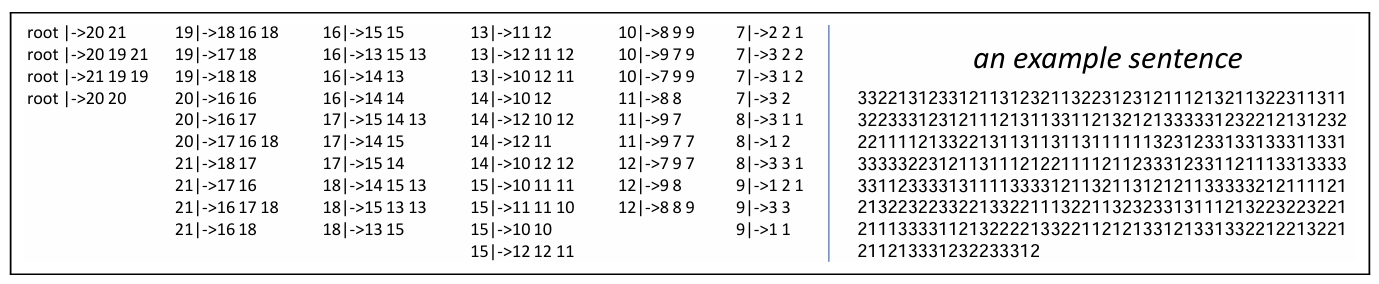
\includegraphics[width=\linewidth]{figures/cfg_example.png}
	
    \caption{\textbf{Left Panel}: CFG rules used in our experiments; \textbf{Right Panel:} an example of the generated sequences using the rules. This figure is taken from \cite{allenzhu2024physicslanguagemodels1}. }
    \label{fig:cfg_example_rule_sequence}
\end{figure*}

\begin{figure*}
    \centering
    \subfigure[]{
        \label{fig:cfg_additional_hier_oe}
		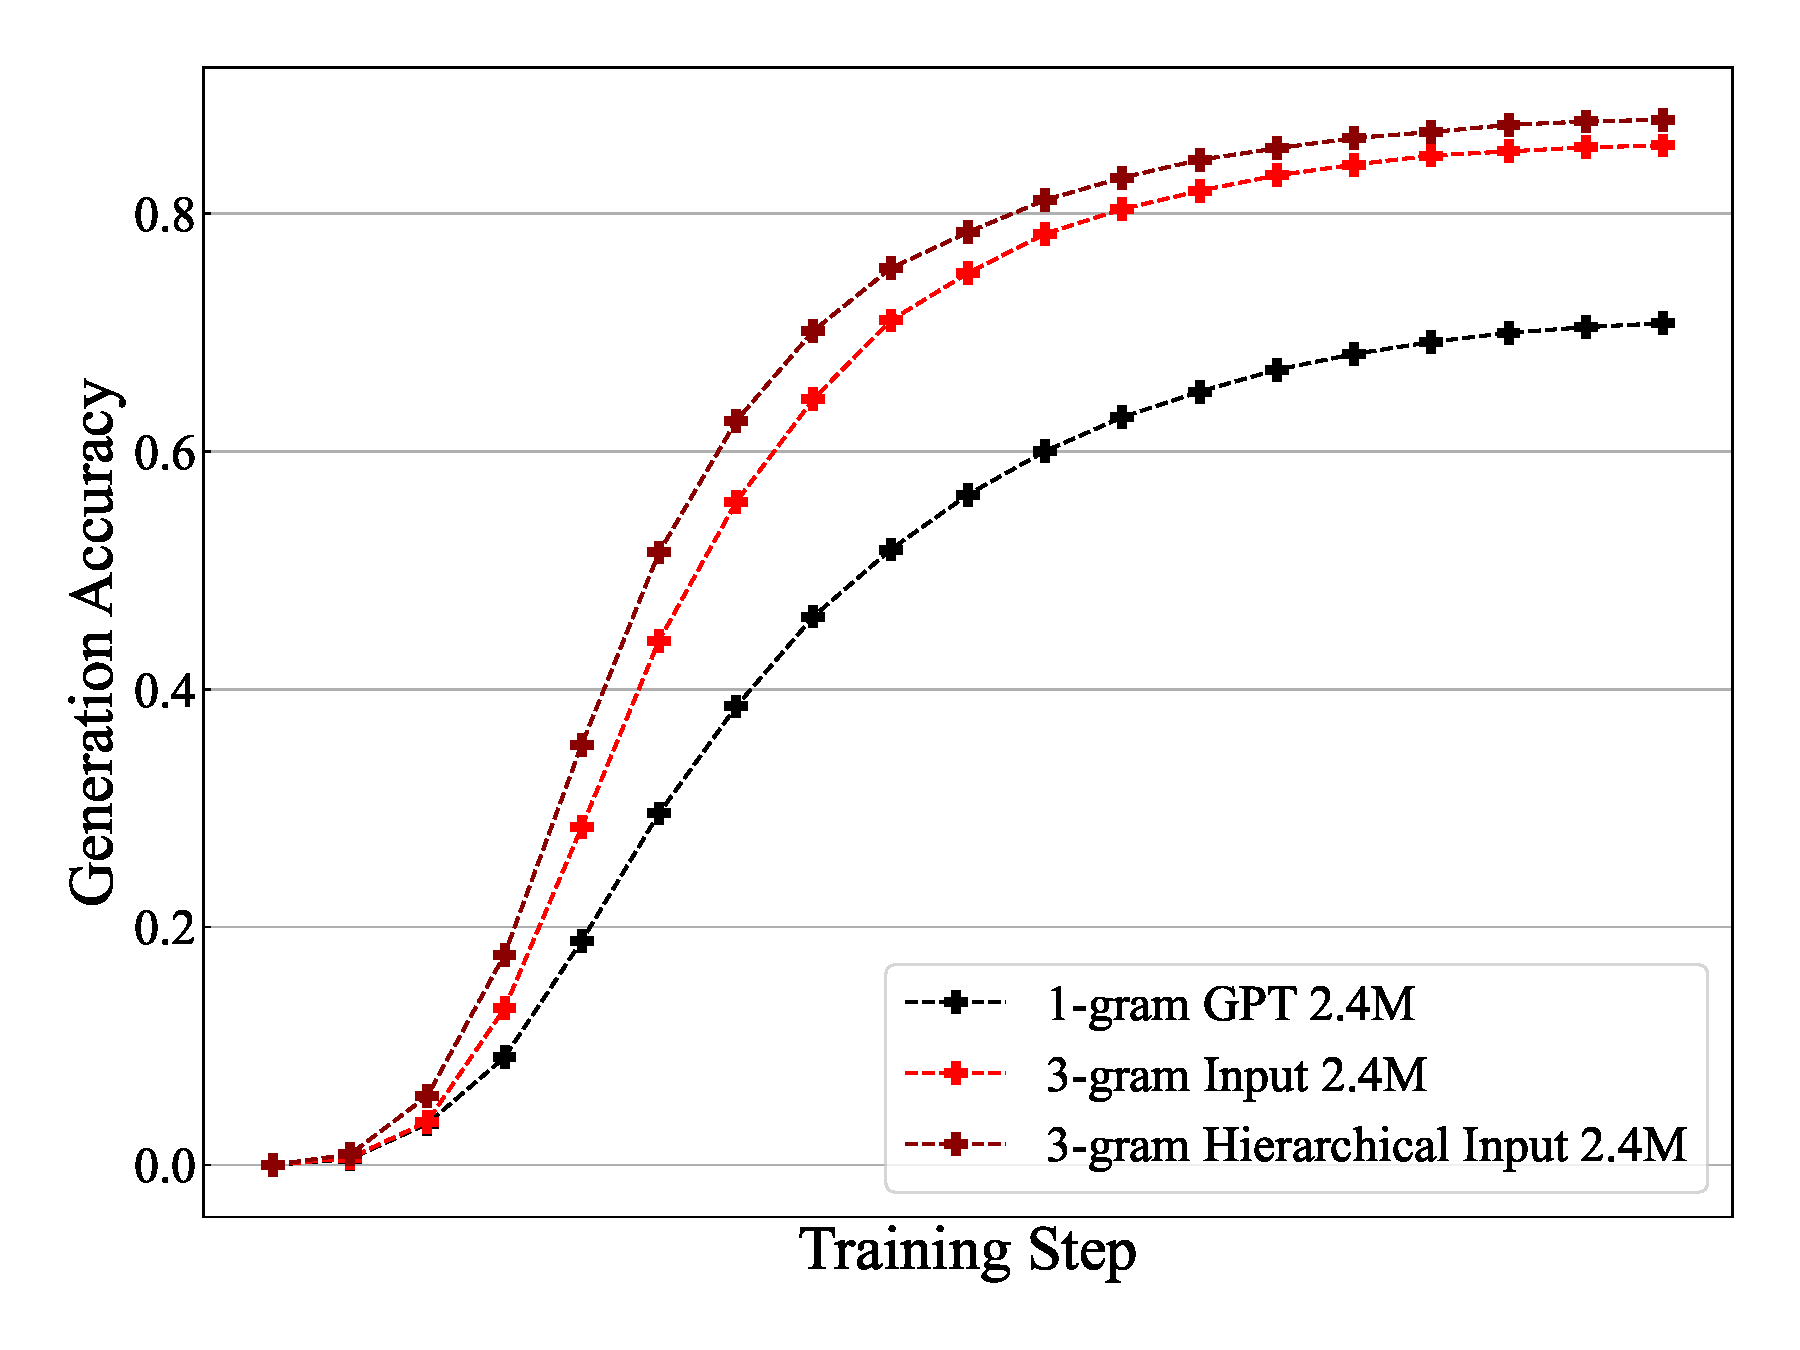
\includegraphics[width=0.31\linewidth]{figures/cfg_hier_overenc.pdf}
	}
 %    \subfigure[]{
 %        \label{fig:cfg_additional_both_oe_od}
	% 	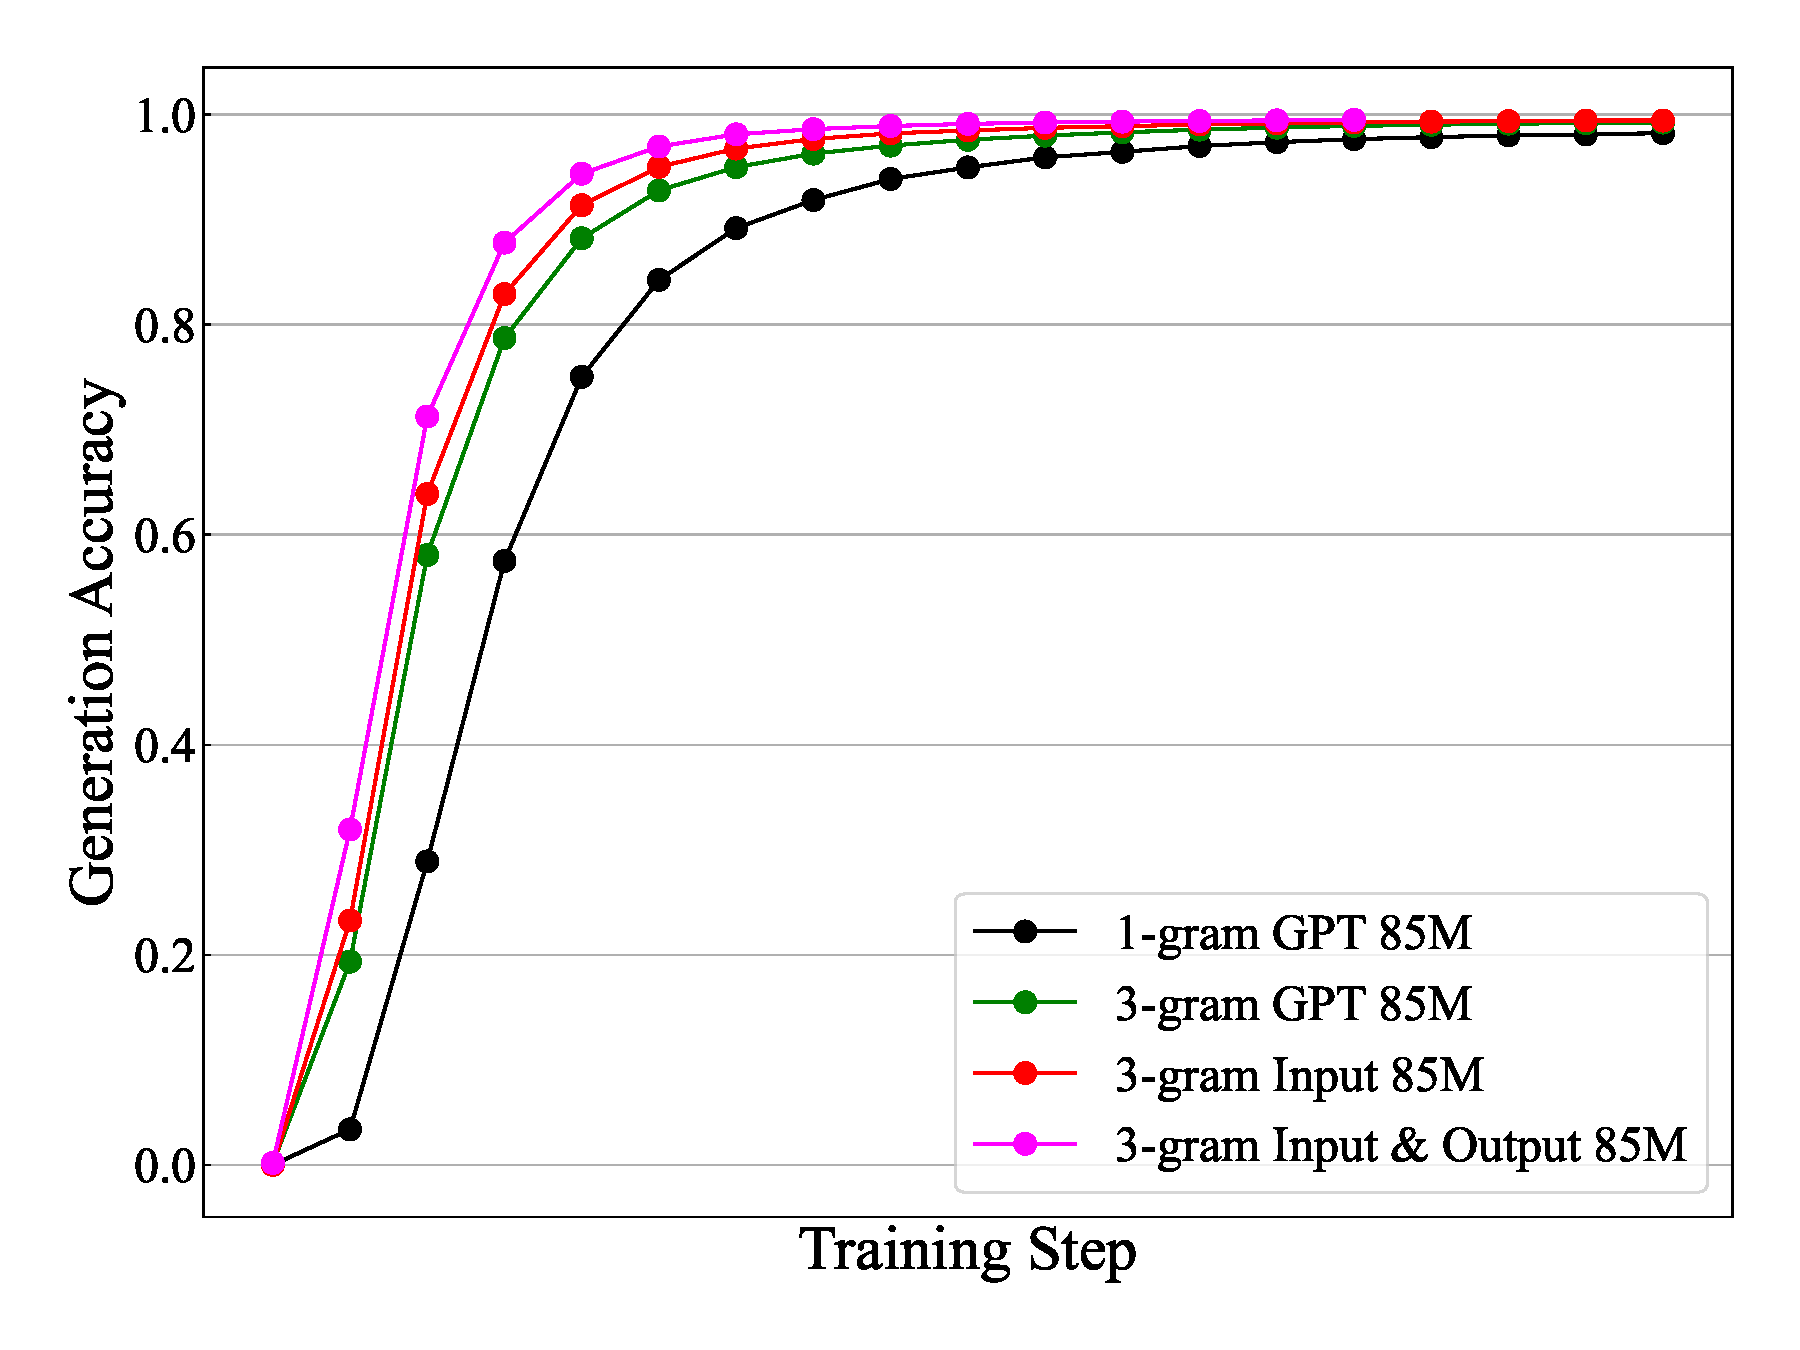
\includegraphics[width=0.48\linewidth]{figures/cfg_overenc_dec.pdf}
	% }
    \subfigure[]{
        \label{fig:cfg_additional_oe_on_2gram_tkn}
		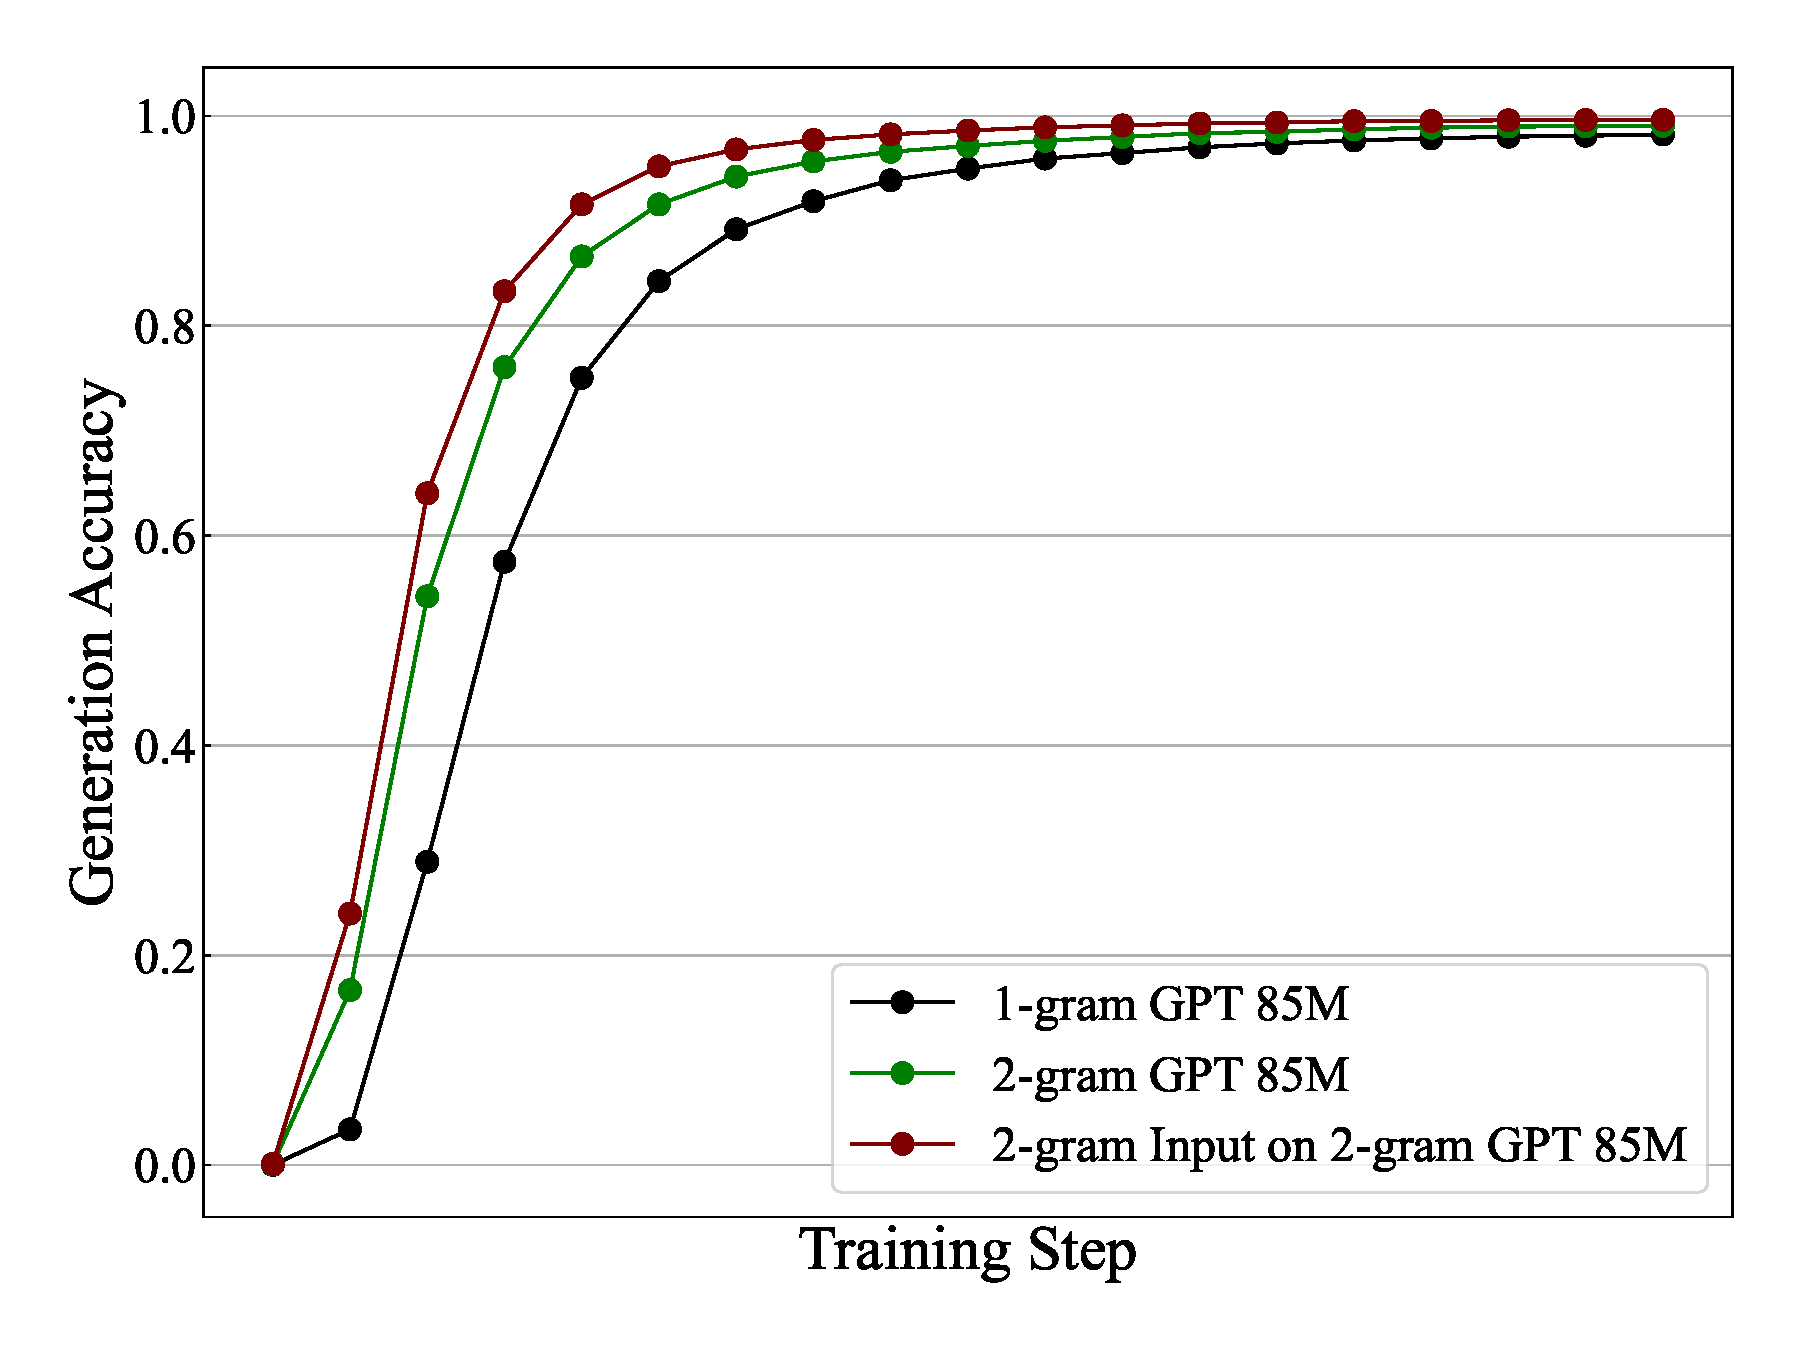
\includegraphics[width=0.31\linewidth]{figures/cfg_oe_on_2gram_tkn.pdf}
	}
    \subfigure[]{
        \label{fig:cfg_additional_oe_on_3gram_tkn}
		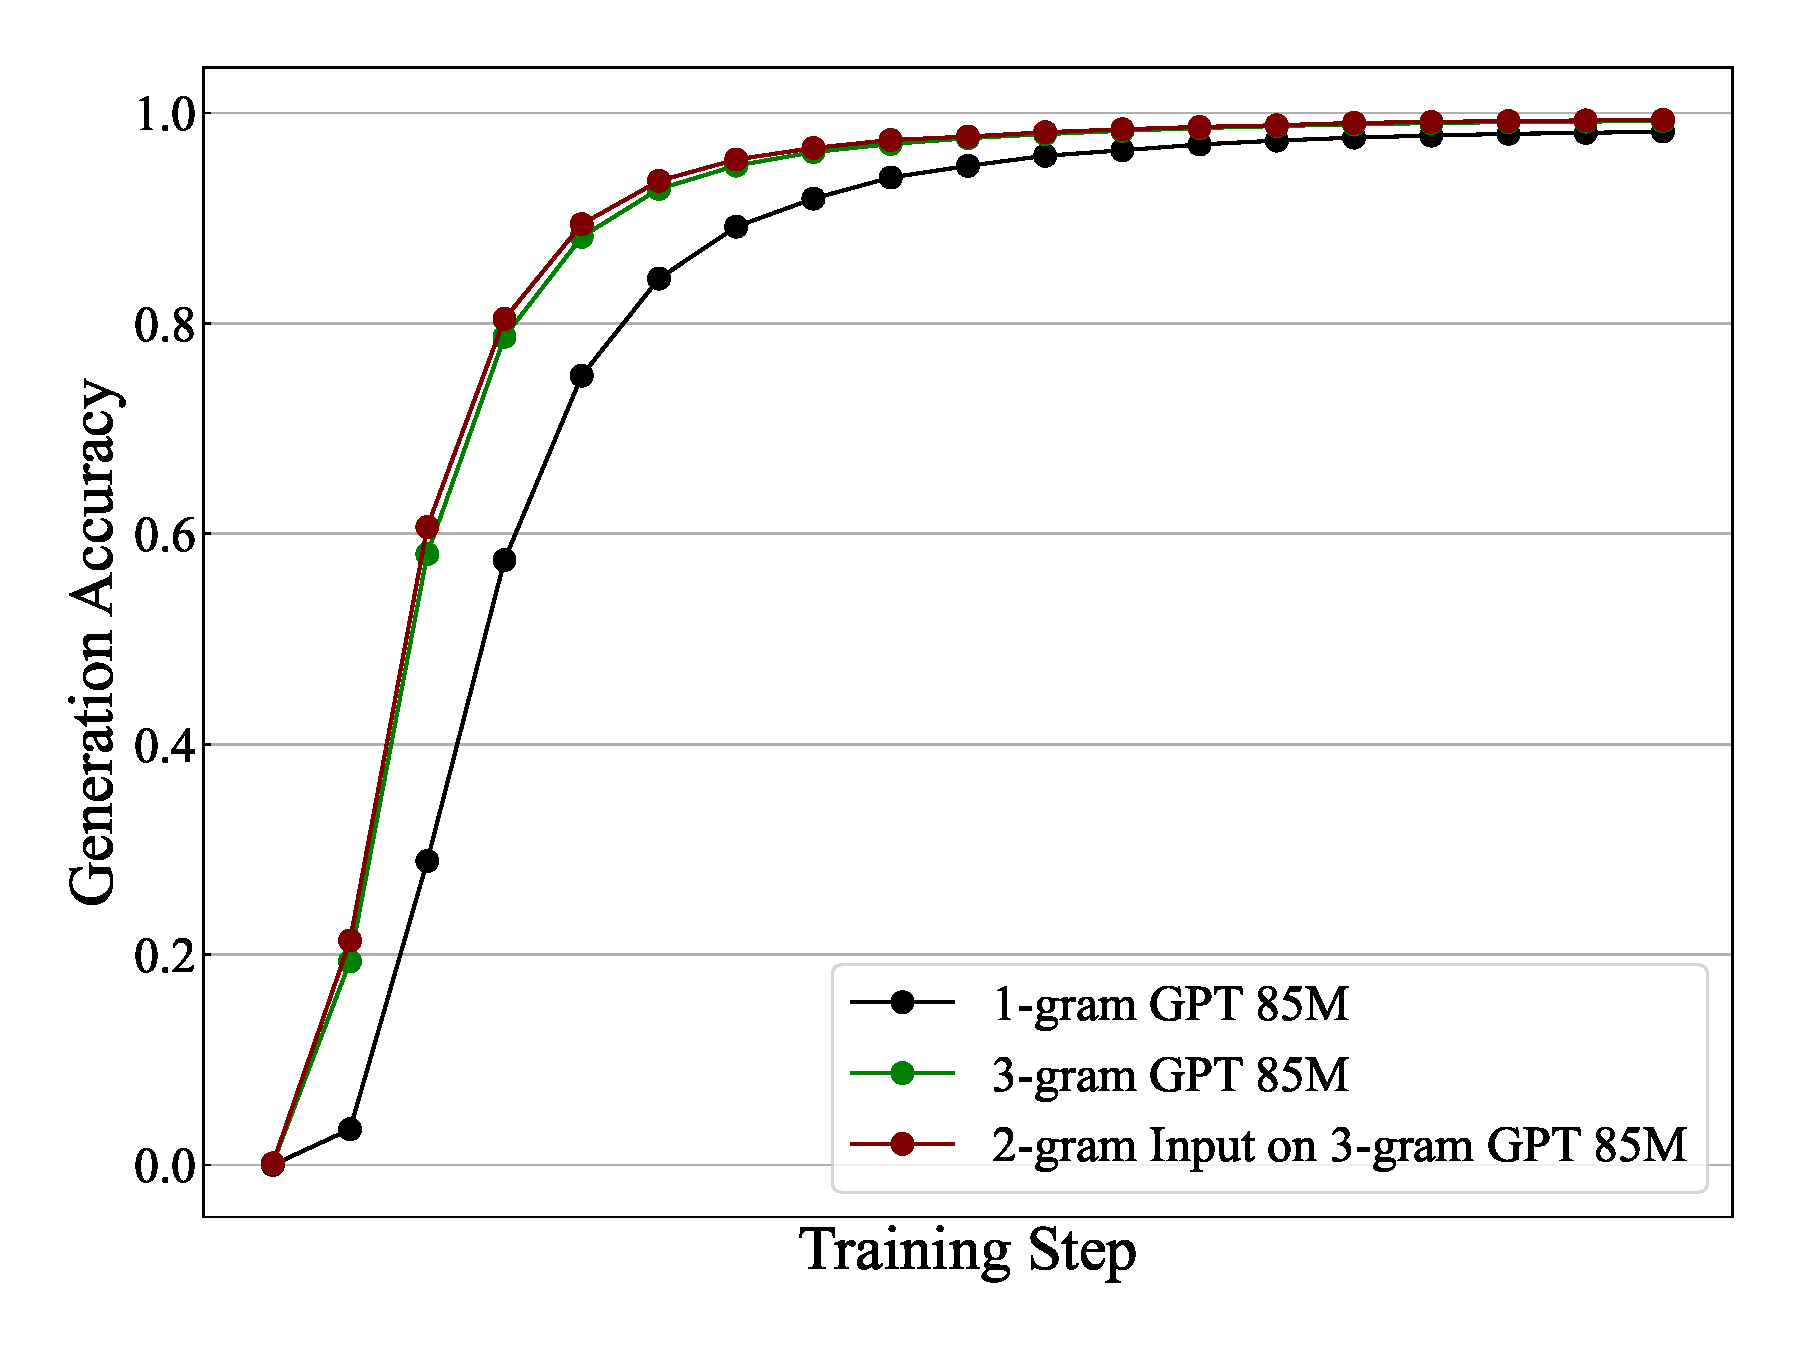
\includegraphics[width=0.31\linewidth]{figures/cfg_oe_on_3gram_tkn.pdf}
	}
    \caption{Performance comparison for models trained on CFG data. }
    \label{fig:cfg_additional_exp}
\end{figure*}


\paragraph{Detailed Setup.} 
We obtain the grammar following \cite{allenzhu2024physicslanguagemodels1} with the configuration named \texttt{cfg3f}, as illustrated in \figref{fig:cfg_example_rule_sequence}. 20 million sentences are sampled from the grammar, serving as a fixed training dataset. We use standard GPT2 architecture, where the larger model uses a hidden size of $768$ and the smaller model $128$. Both larger and smaller models have 12 transformer layers, as depth is discovered essential to complex CFG modeling~\cite{allenzhu2024physicslanguagemodels1}. We use AdamW optimizer with $\beta=(0.9, 0.98)$, weight decay 0.1, initial learning rate $3e^{-4}$ and batch size $64\times8$. The models are trained with cosine learning rate scheduler for 10 epoch. To evaluate model performance, we 10,000 sample sentences from the trained model auto-regressively using the raw next token probability. The sentences are then verified by the ground-truth grammar, and the ratio of accurate samples is denoted as generation accuracy.

\paragraph{Implementation of $n$-gram tokenization or over-tokenization.} Though we mentioned a $3^n$-sized vocabulary for $n$-gram tokenization or $n$-gram over-tokenization in the main text, the actual vocabulary should be $2+\sum_{i=1}^n3^i$. The bias $2$ stands for the BOS(Begin Of Sequence) and EOS(End of Sequence) token and extra $3^i$ terms are for the corner cases where the sequence length may not be divisible by $n$. We refer to $3^n$-sized vocabulary in the main text primarily to emphasize the order of magnitude.

\paragraph{Hierarchical $n$-gram input further improves.} 
We experiment with introducing hierarchical $n$-gram inputs in the CFG setting. Initially, we use a single $V^n$-size $n$-gram embedding table to handle the model's input. To consider hierarchical $n$-gram modeling, we add $n-1$ additional embedding tables, where the $i$-th table has a size of $V^i$, and use $i$-gram token as input. Notably, the parameters of these $n-1$ embedding tables can be fully merged into the $n$-gram embedding table, so the effective parameter count does not increase. Instead, this process re-parameterizes the embedding table to decompose parameters hierarchically. 
The experimental results, shown in \figref{fig:cfg_additional_hier_oe}, indicate that the model with hierarchically decomposed 3-gram inputs outperforms the model with naive 3-gram inputs. This further validates that even for models with a complete $n$-gram vocabulary (rather than approximated through matrix decomposition), hierarchically modeling multi-granularity tokens remains highly effective.

\paragraph{Ablation on base tokenizers. } We replaced the base tokenizer to investigate whether further increasing the input vocabulary size could lead to additional improvements. Specifically, we expanded the input vocabulary for 2-gram and 3-gram base tokenizers to 2-gram inputs with vocabulary sizes of $(3^2)^2 = 81$ and $(3^3)^2 = 729$, respectively. The experimental results, shown in \figref{fig:cfg_additional_oe_on_2gram_tkn} and \figref{fig:cfg_additional_oe_on_3gram_tkn}, demonstrate that increasing the input vocabulary consistently improves model performance. 
Another observation is that, when using the 3-gram base tokenizer, the benefit of increased convergence speed from 2-gram inputs becomes notably smaller. We hypothesize that this is related to the ``slow-start" nature of large vocabularies. Similar observations have been made in natural language processing, where larger input vocabularies require more training tokens to realize their expected benefits.

\subsection{OLMo2 Experiments}
\label{sec:appendix_detailed_olom2_exps}

\paragraph{Detailed metrics.} We present a detailed training dynamics comparison for models on OLMo2-1B in \figref{fig:olmoe_1b3_oe_all_metrics}. OE achieves significant improvements across most metrics, while maintaining at least parity on the remaining ones.



\begin{figure*}
    \centering
    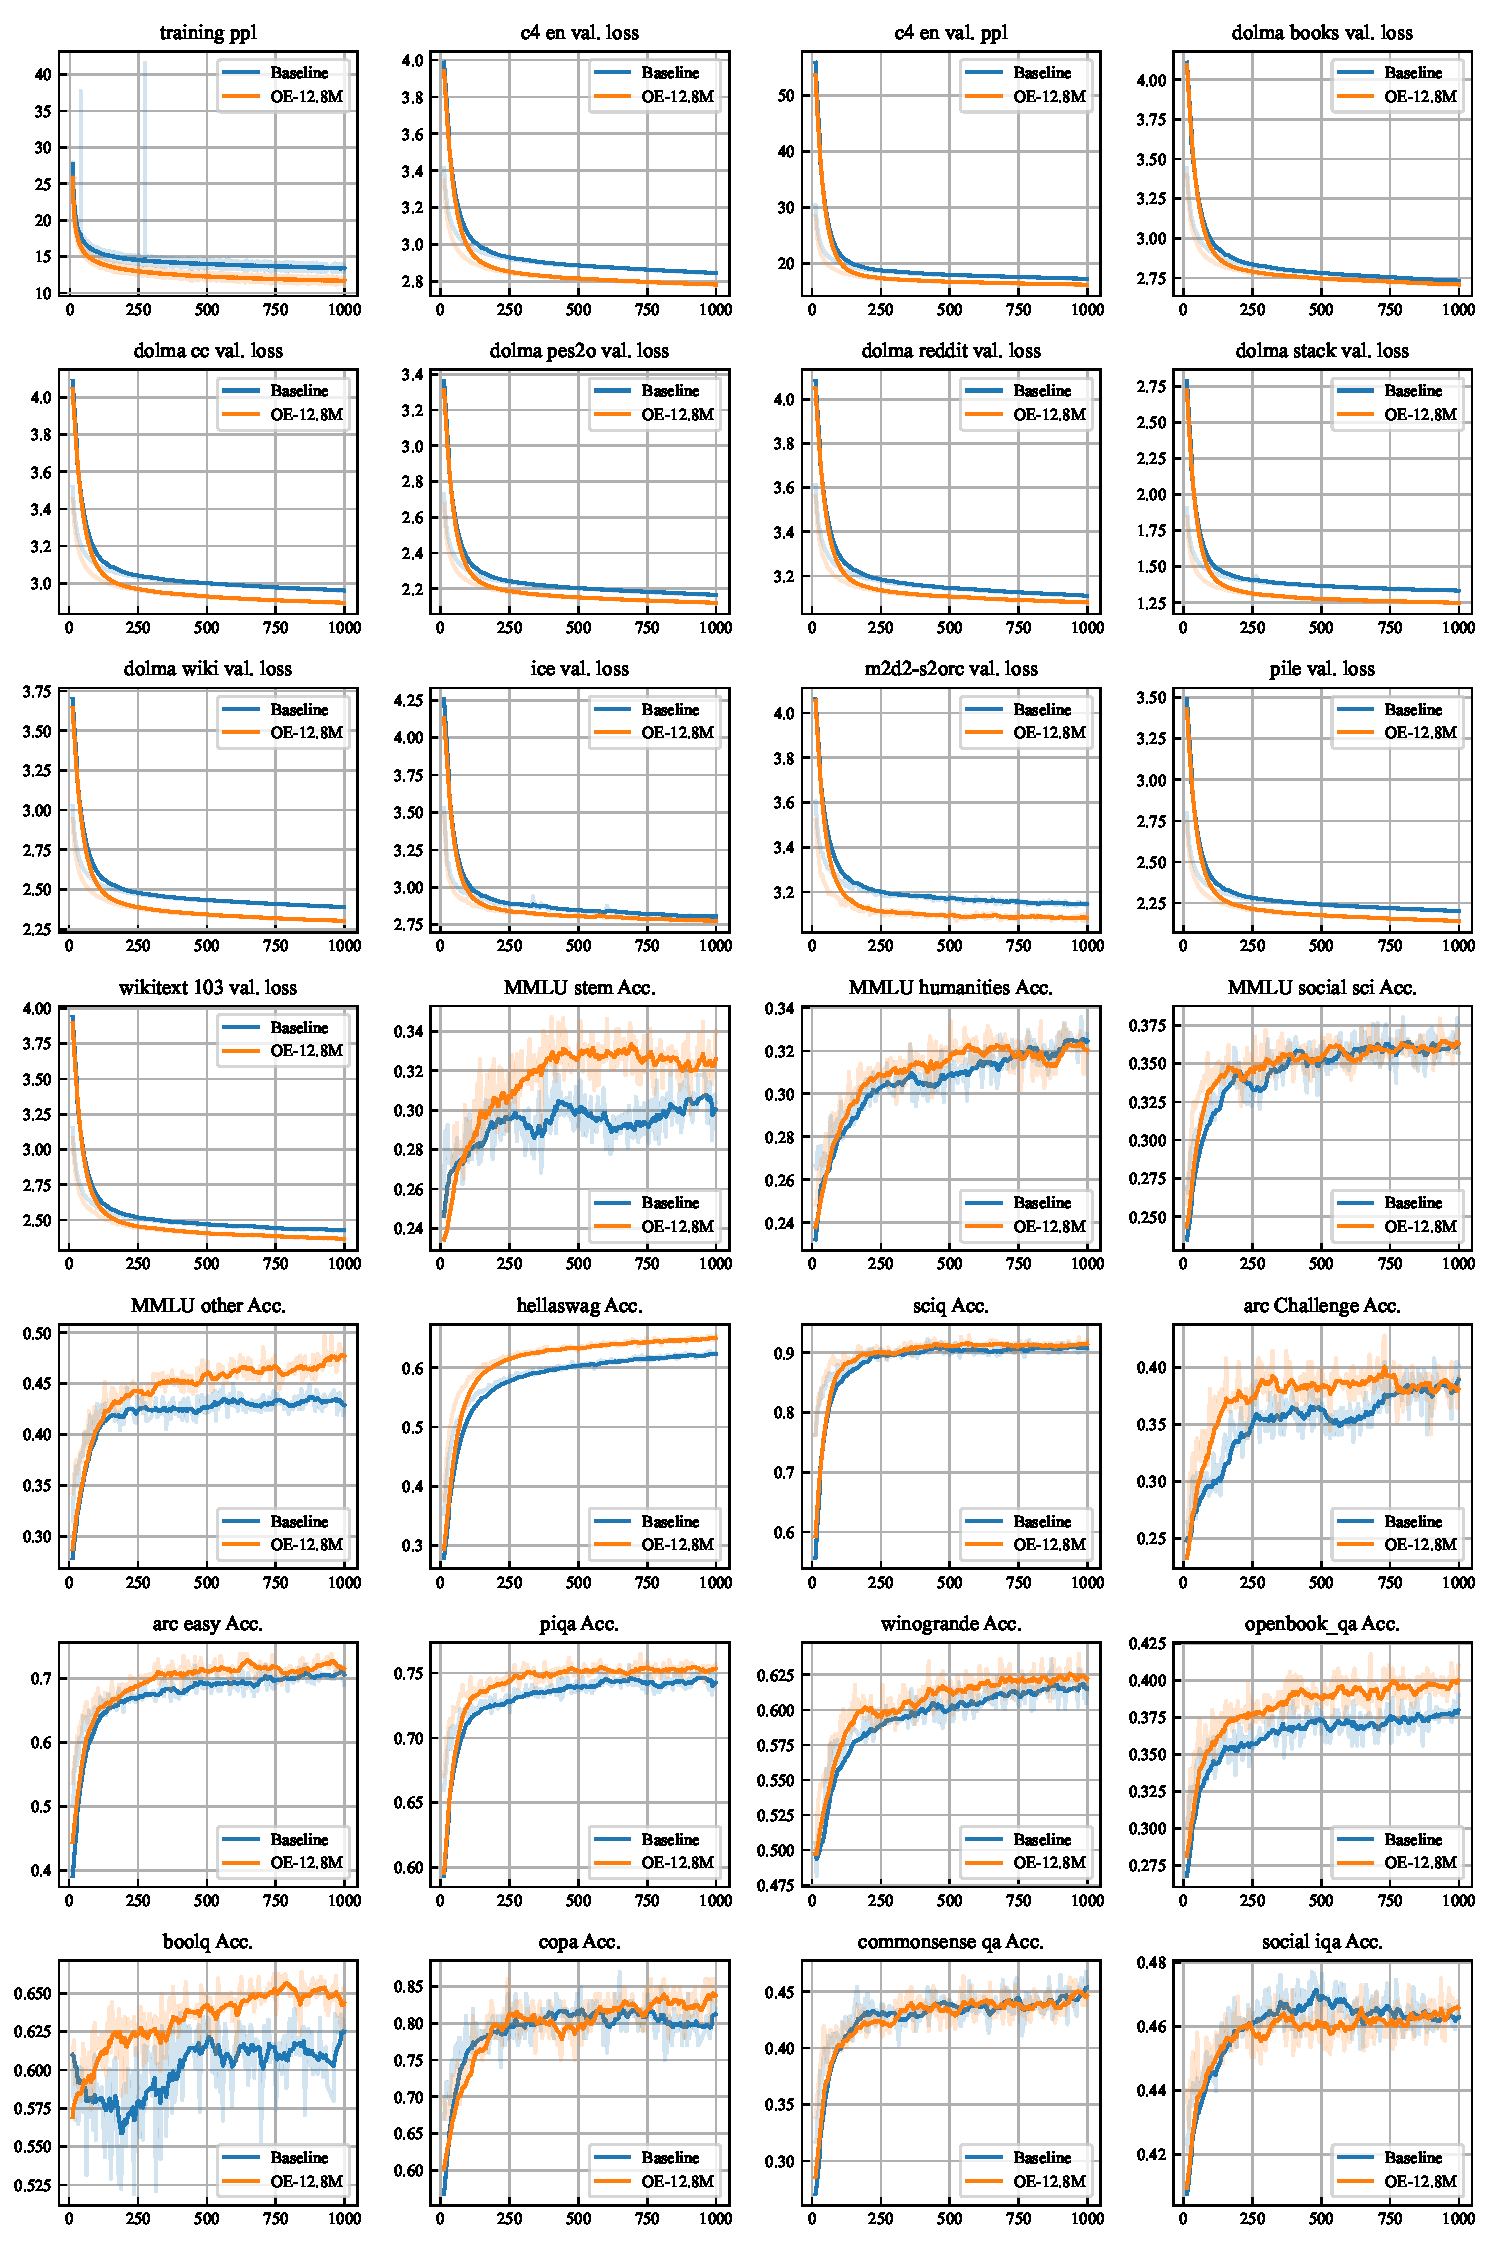
\includegraphics[width=0.85\linewidth]{figures/olmo2_1b_oe_all_metrics.pdf}
    \caption{All metrics for OLMo2-1B, comparing OE-12.8M and baseline. }
    \label{fig:olmoe_1b3_oe_all_metrics}
\end{figure*}



\subsection{OLMoE Experiments}
\label{sec:appendix_detailed_olome_exps}


\begin{figure*}
    \centering
    \subfigure[Loss Curves]{
        \label{fig:}
	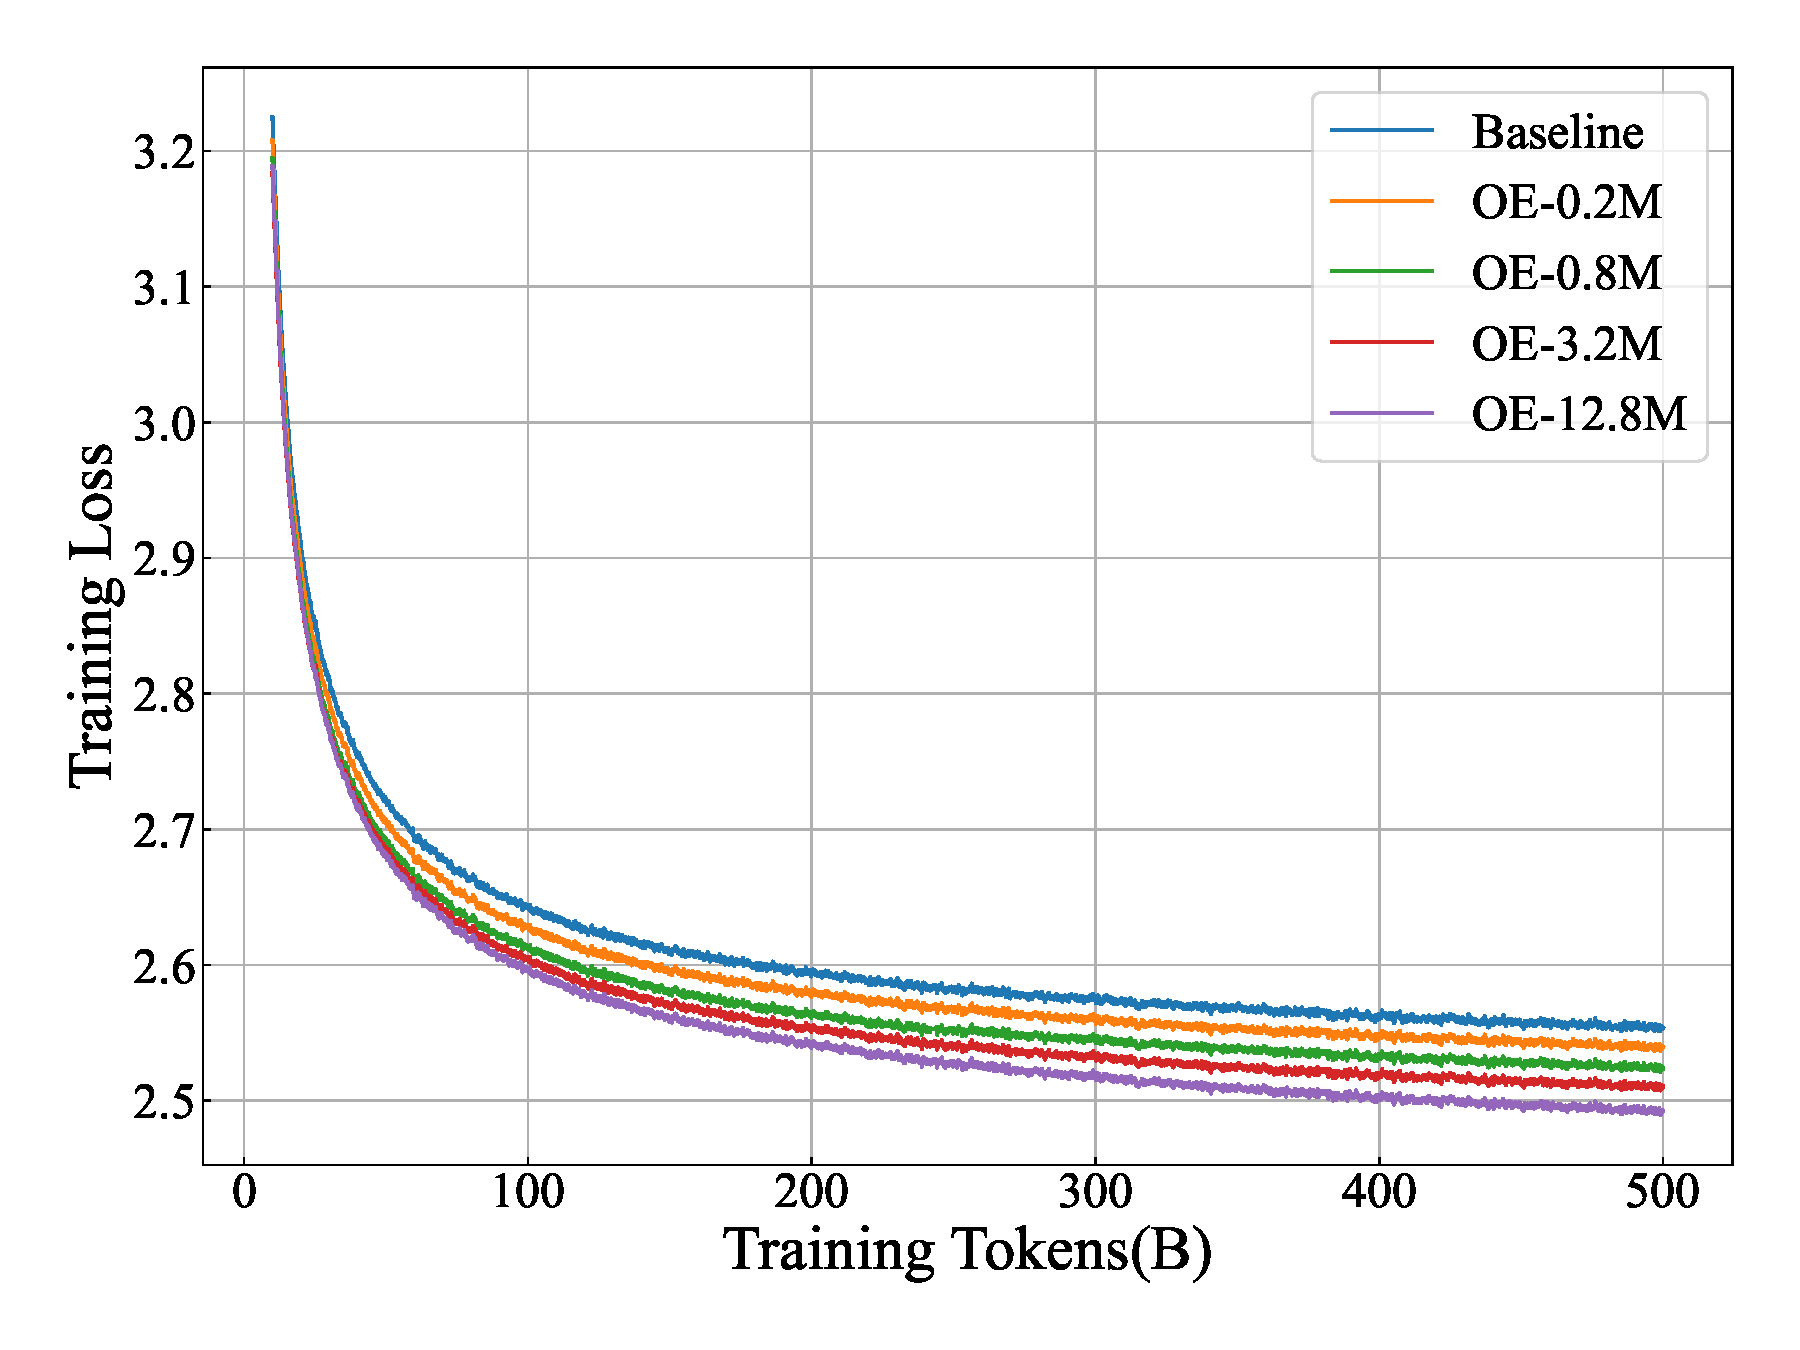
\includegraphics[width=0.45\linewidth]{figures/olmoe_scaling_vocab_losscurve.pdf}
	}
    \subfigure[Loss Diff]{
        \label{fig:}
	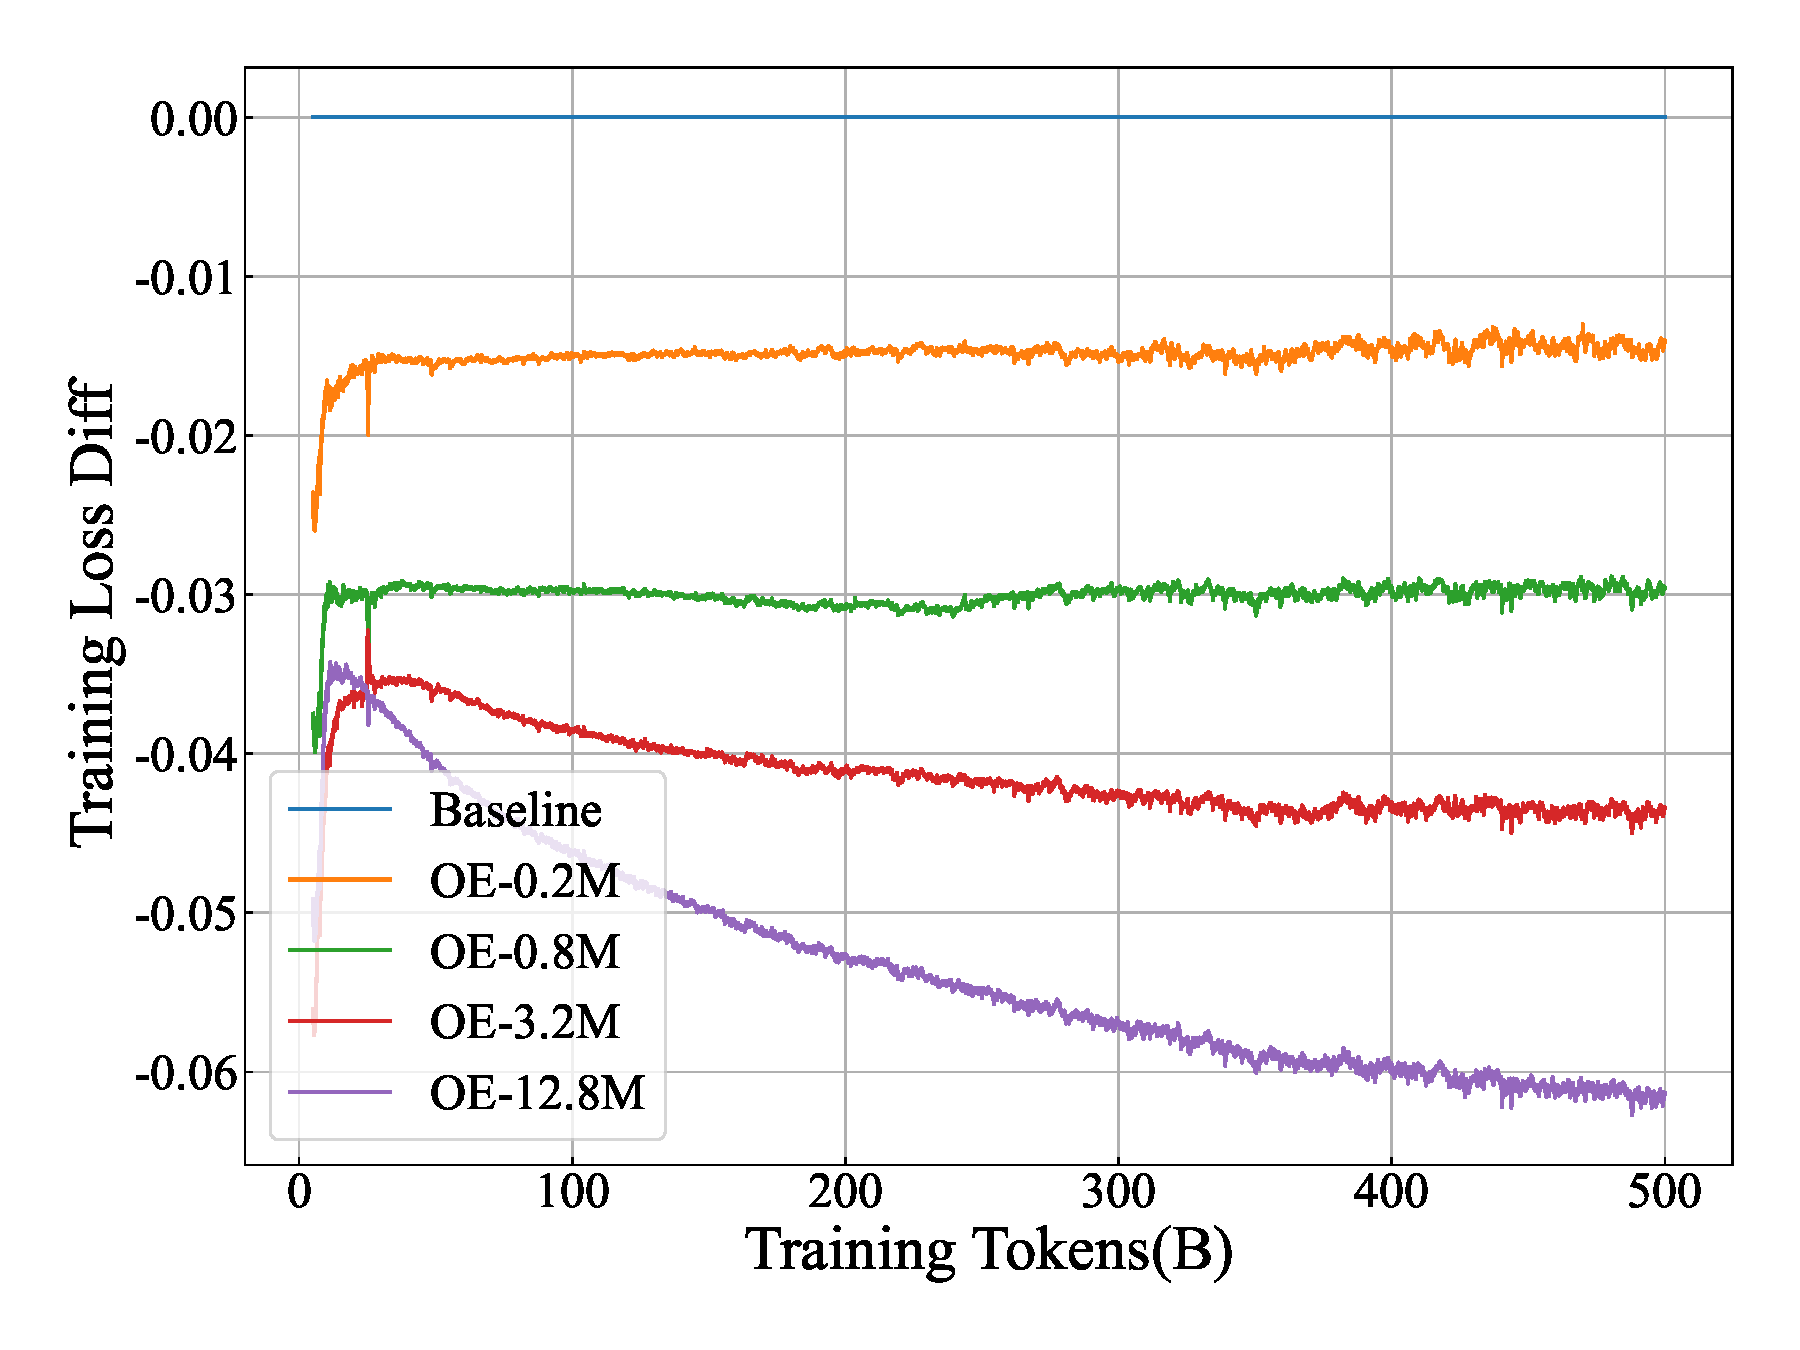
\includegraphics[width=0.45\linewidth]{figures/olmoe_scaling_vocab_losscurve_diff.pdf}
	}
    \caption{Loss curves for vocabulary scaling experiments, where OE models use the setting of $n=2, k=1$. The curves are smoothed with exponential moving average of weight $0.99$. }
    \label{fig:olmoe_scaling_vocab_loss_curves}
\end{figure*}

\begin{figure*}
    \centering
    \subfigure[Loss Curves]{
        \label{fig:}
	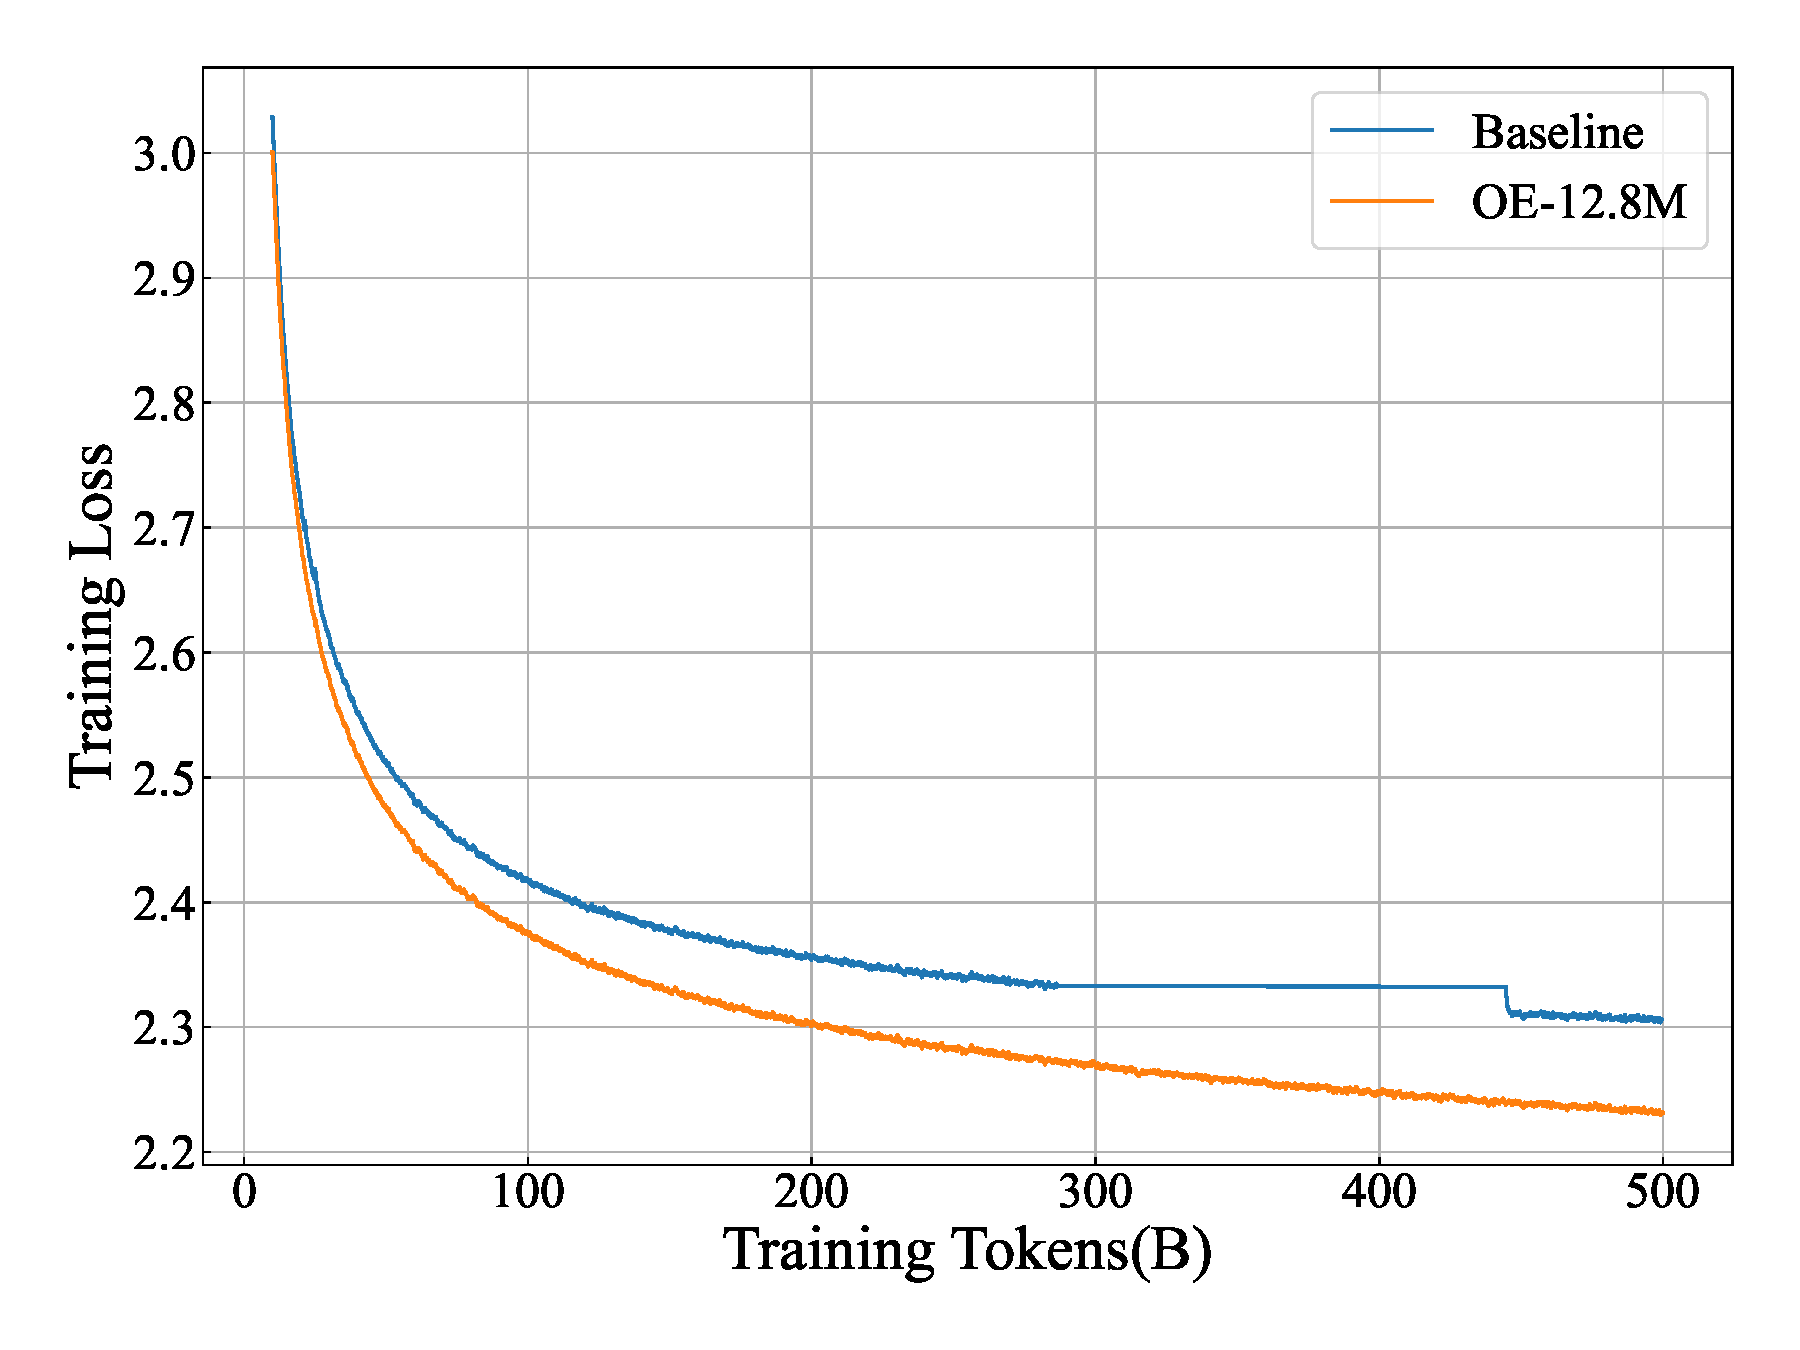
\includegraphics[width=0.45\linewidth]{figures/olmoe_sota_7b_oe_TrainingLoss.pdf}
	}
    \subfigure[Loss Diff]{
        \label{fig:}
	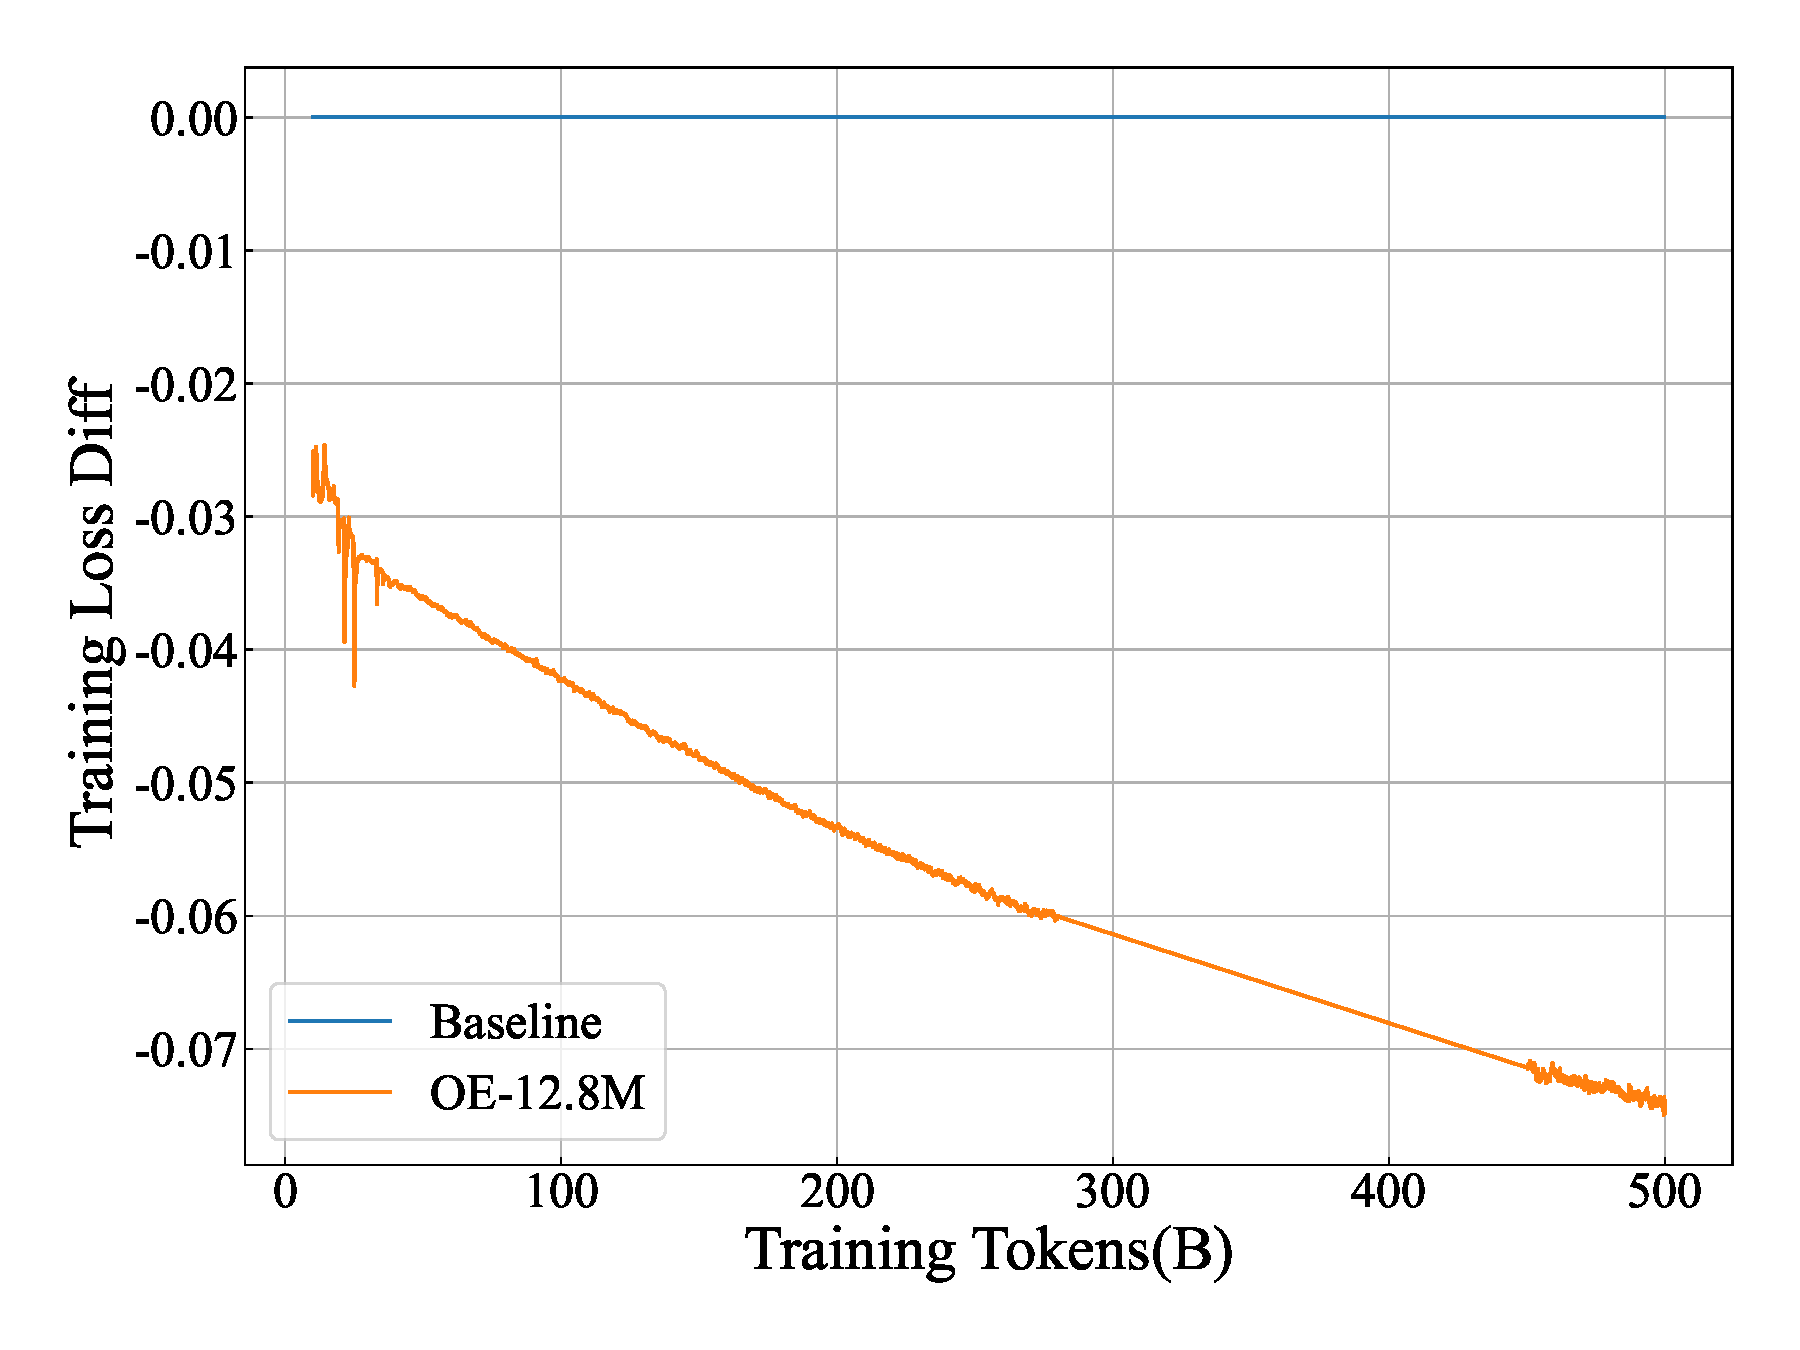
\includegraphics[width=0.45\linewidth]{figures/olmoe_sota_7b_oe_TrainingLoss_diff.pdf}
	}
    \caption{Loss curves for OLMoE-7B experiments. The OE model uses the setting of $n=3, k=4$. The curves are smoothed with exponential moving average of weight $0.99$. The flat part in baseline is a consequence of wandb log missing. }
    \label{fig:olmoe_7b_sota_loss_curves}
\end{figure*}

\begin{figure*}
    \centering
    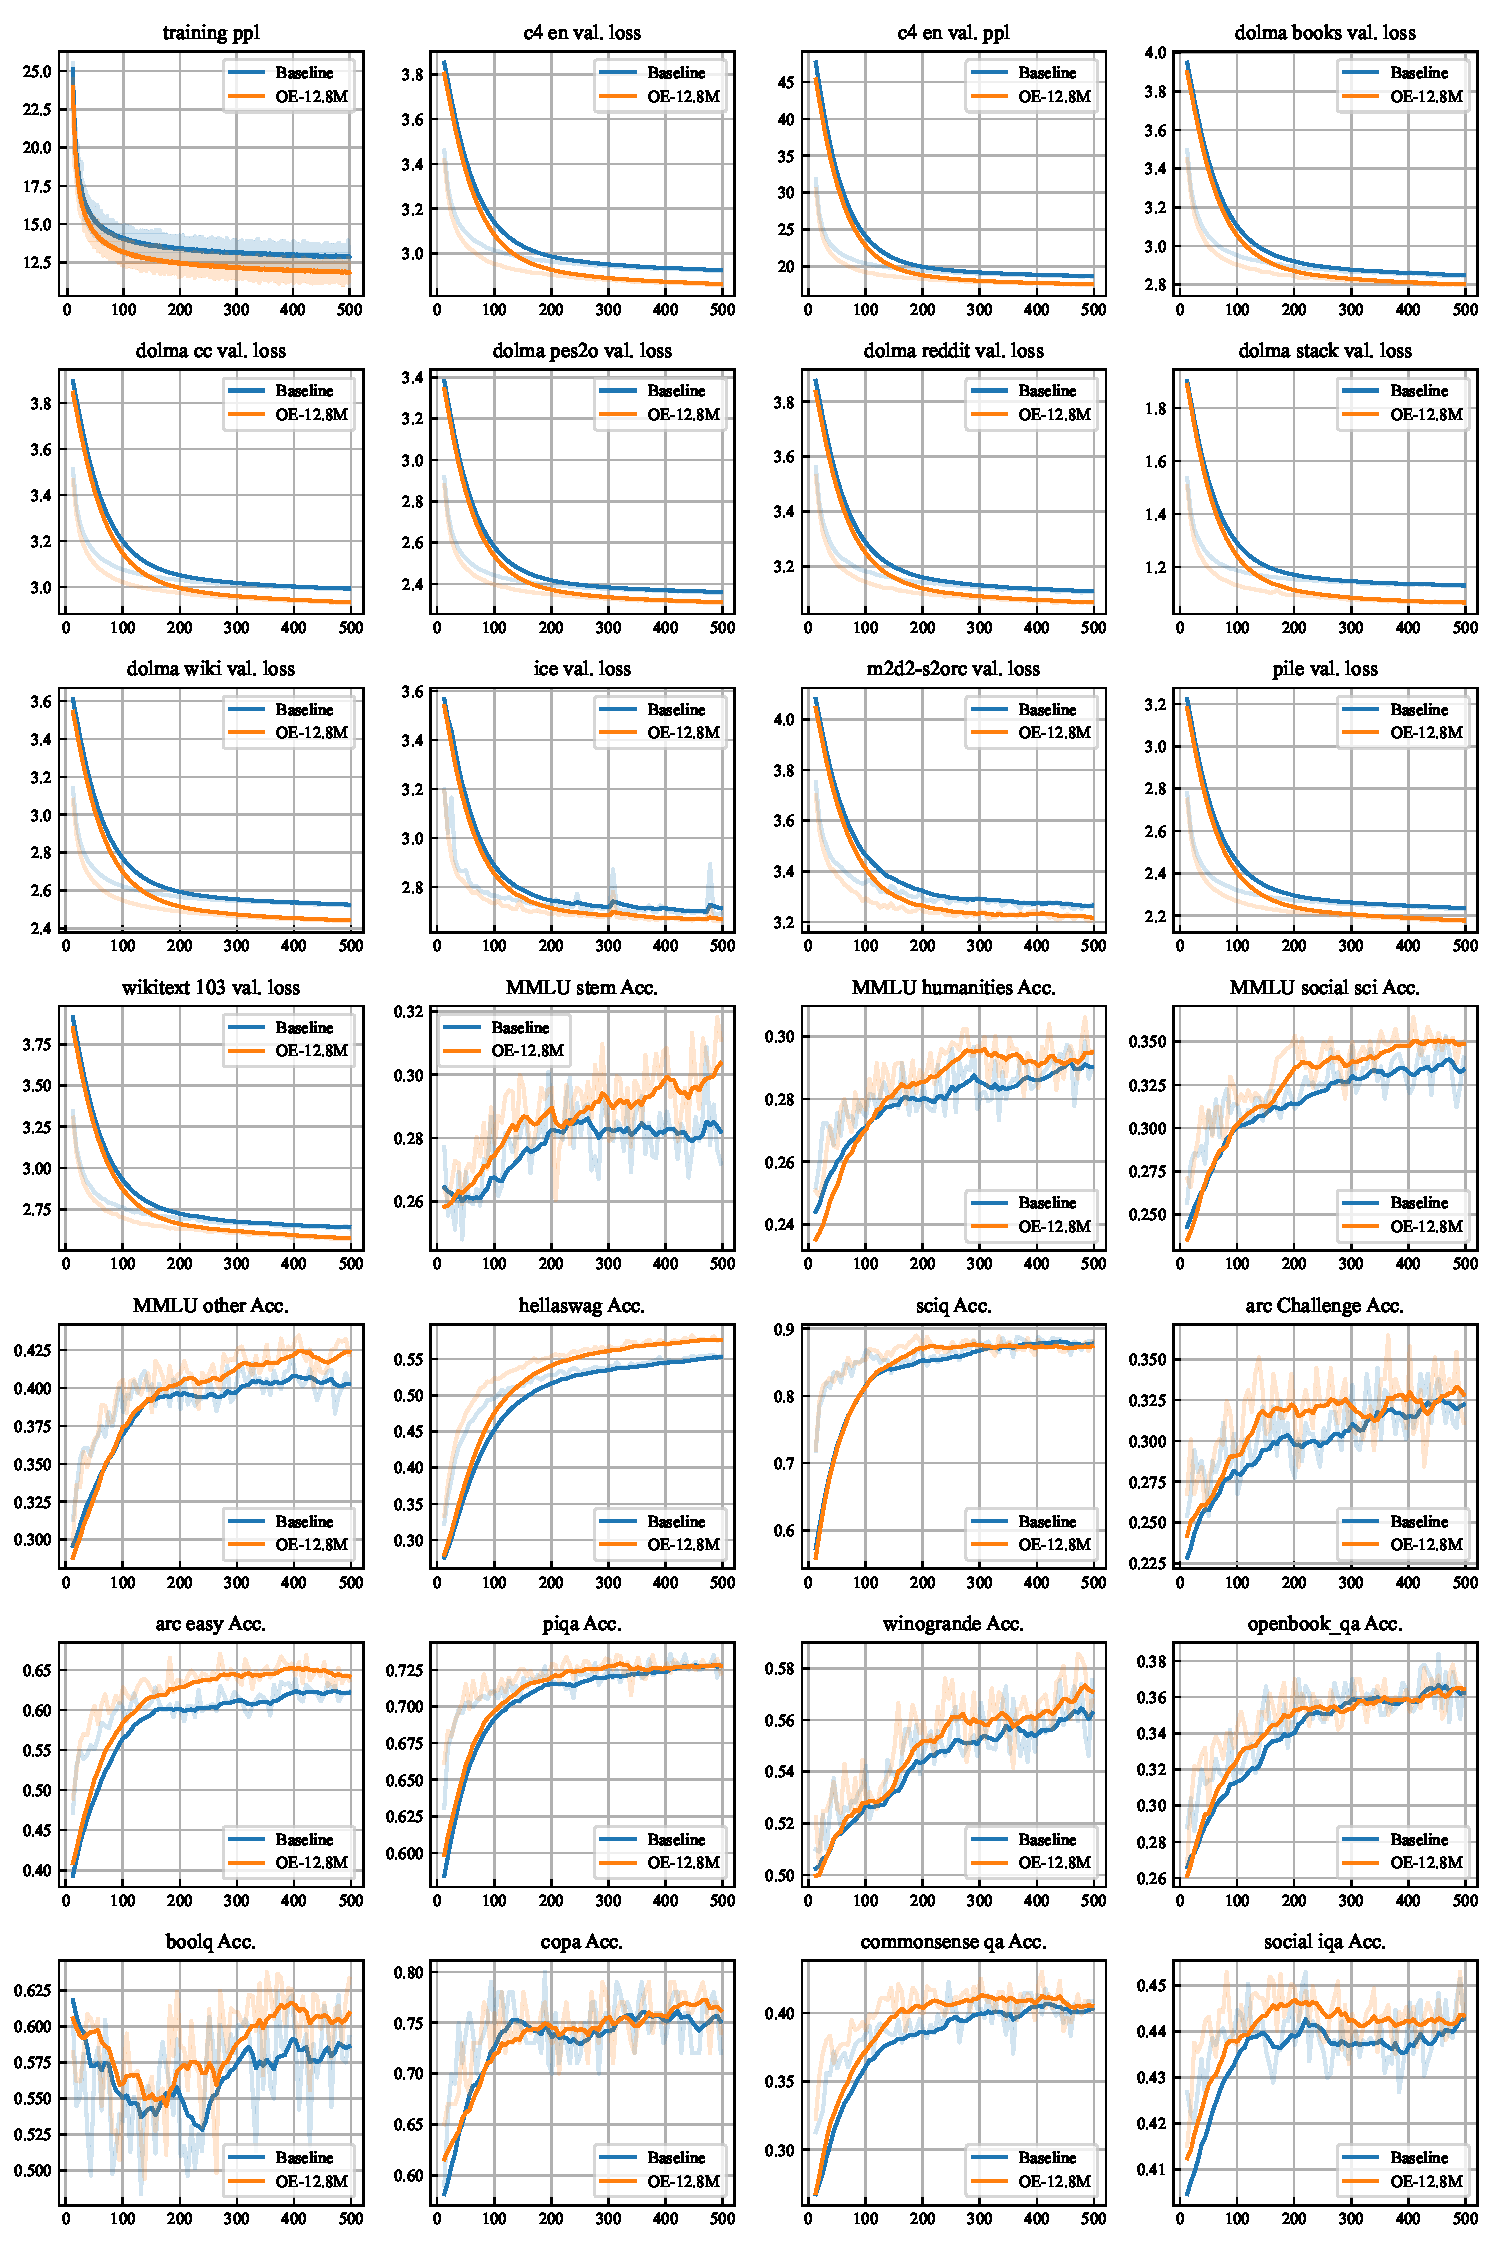
\includegraphics[width=0.85\linewidth]{figures/olmoe_1b3_oe_all_metrics.pdf}
    \caption{All metrics for OLMoE-1.3B, comparing OE-12.8M and baseline. }
    \label{fig:olmoe_1b3_oe_all_metrics}
\end{figure*}

\begin{figure*}
    \centering
    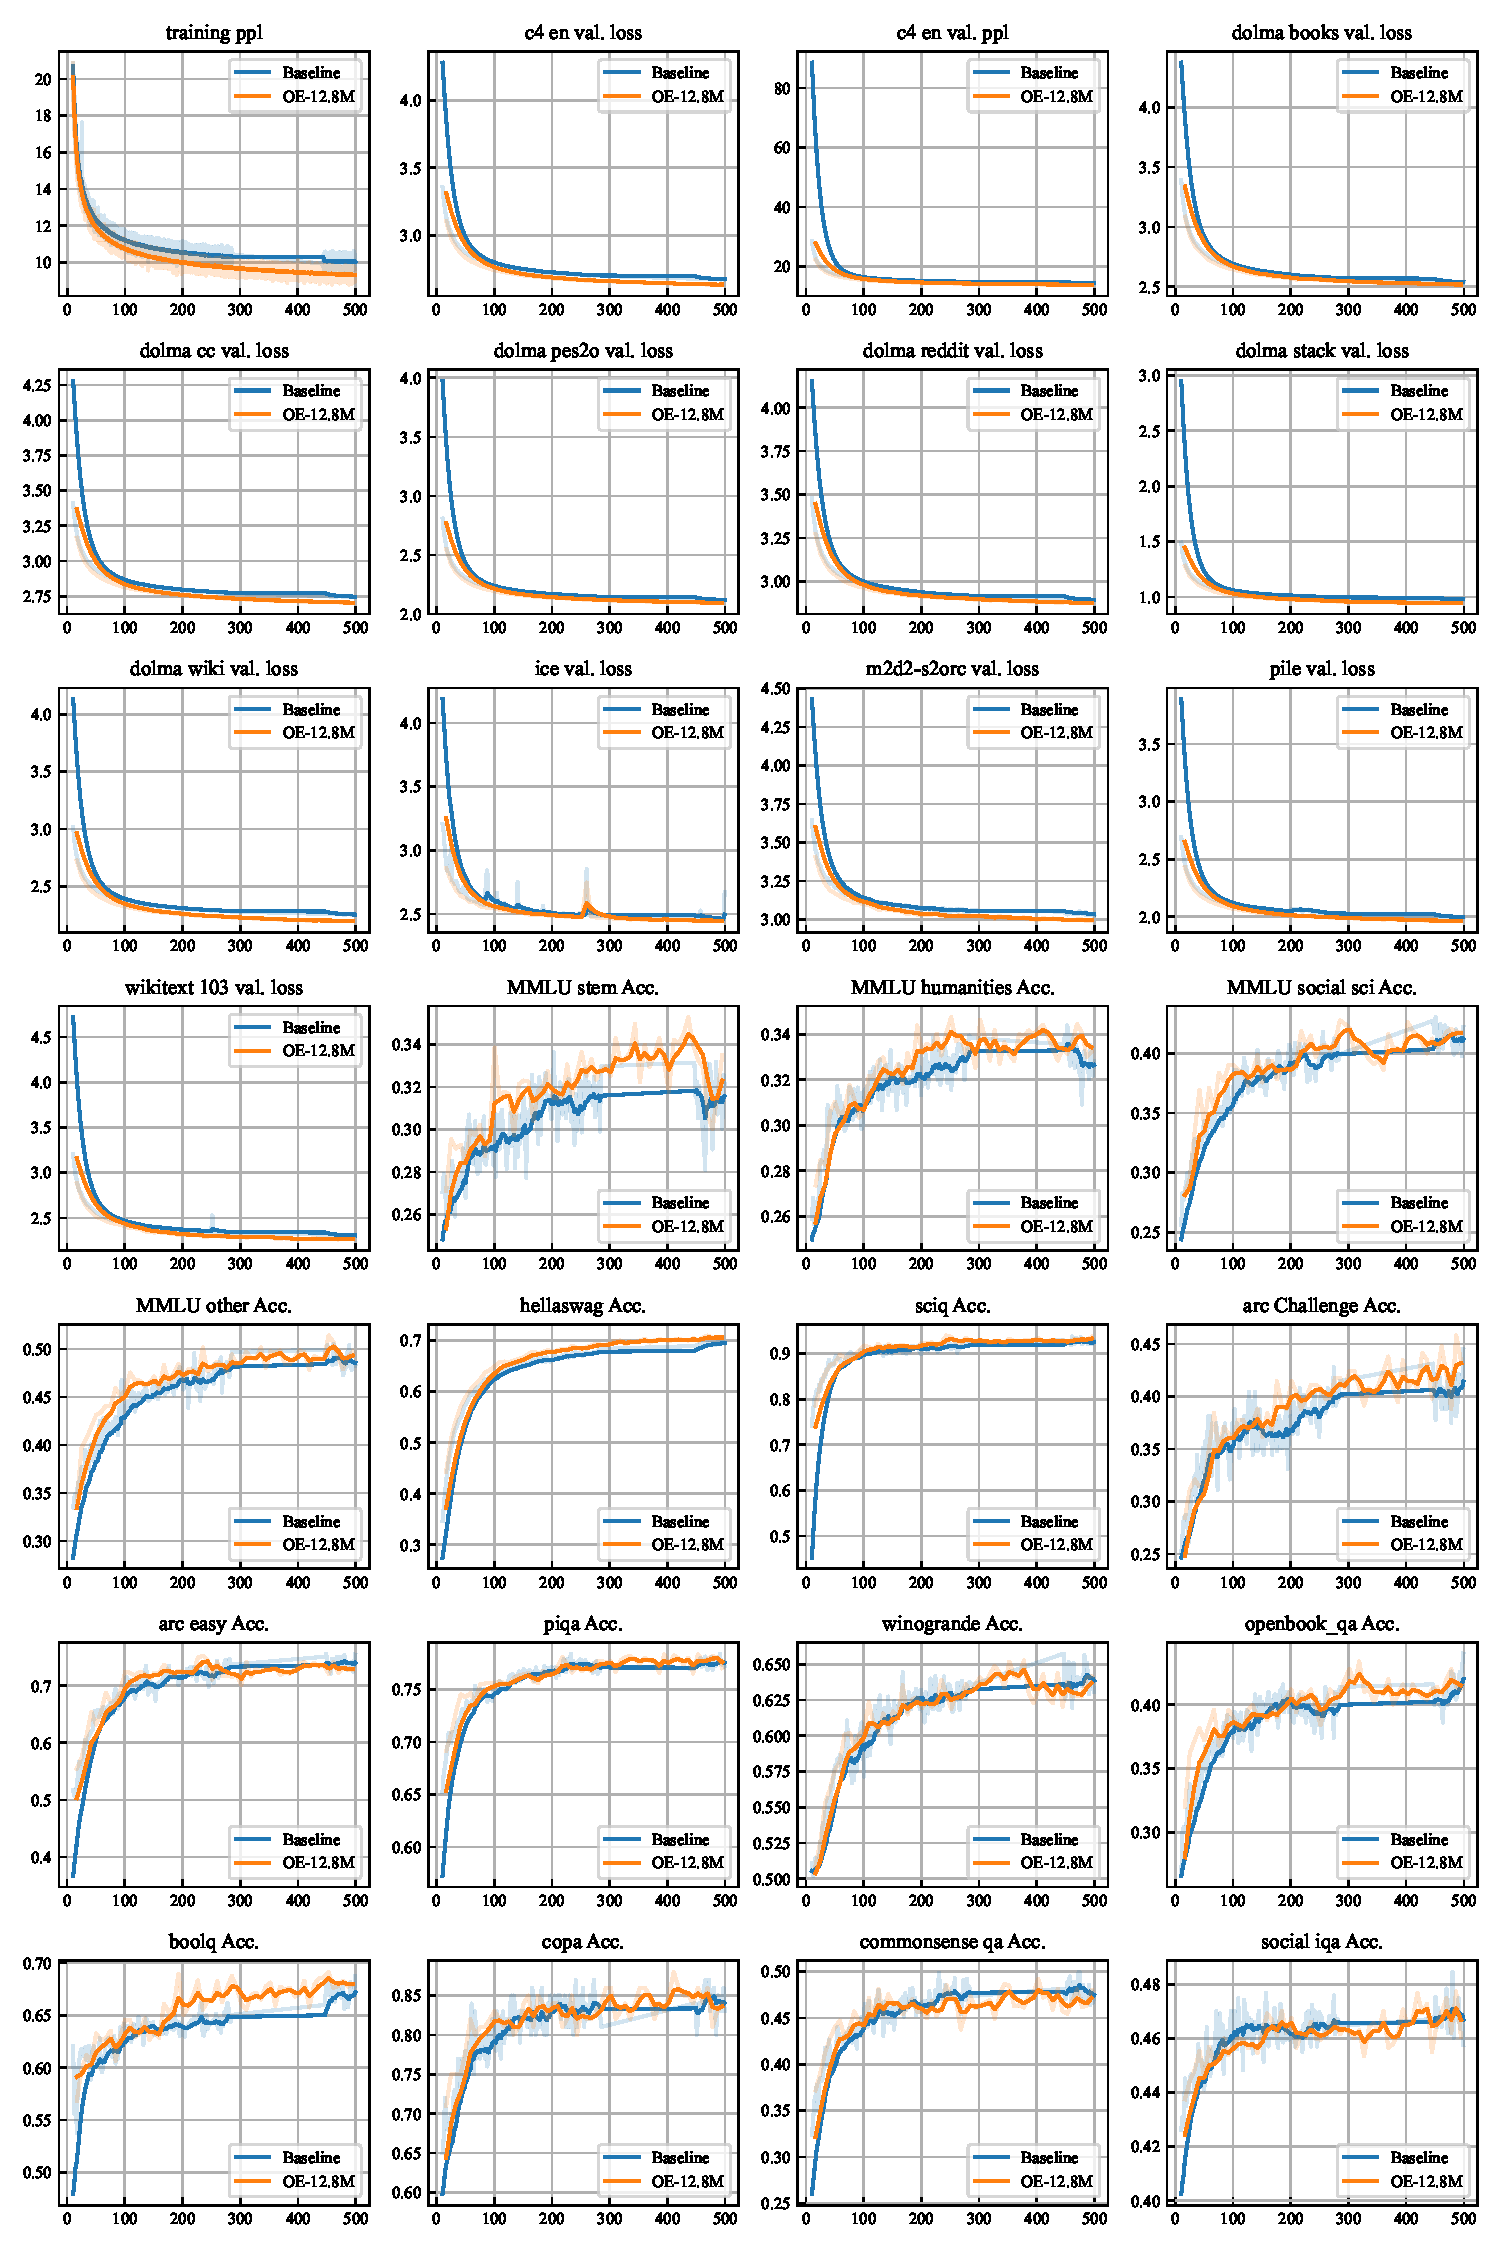
\includegraphics[width=0.85\linewidth]{figures/olmoe_7b_oe_all_metrics.pdf}
    \caption{All metrics for OLMoE-7B, comparing OE-12.8M and baseline. }
    \label{fig:olmoe_7b_oe_all_metrics}
\end{figure*}

\begin{figure*}
    \centering
    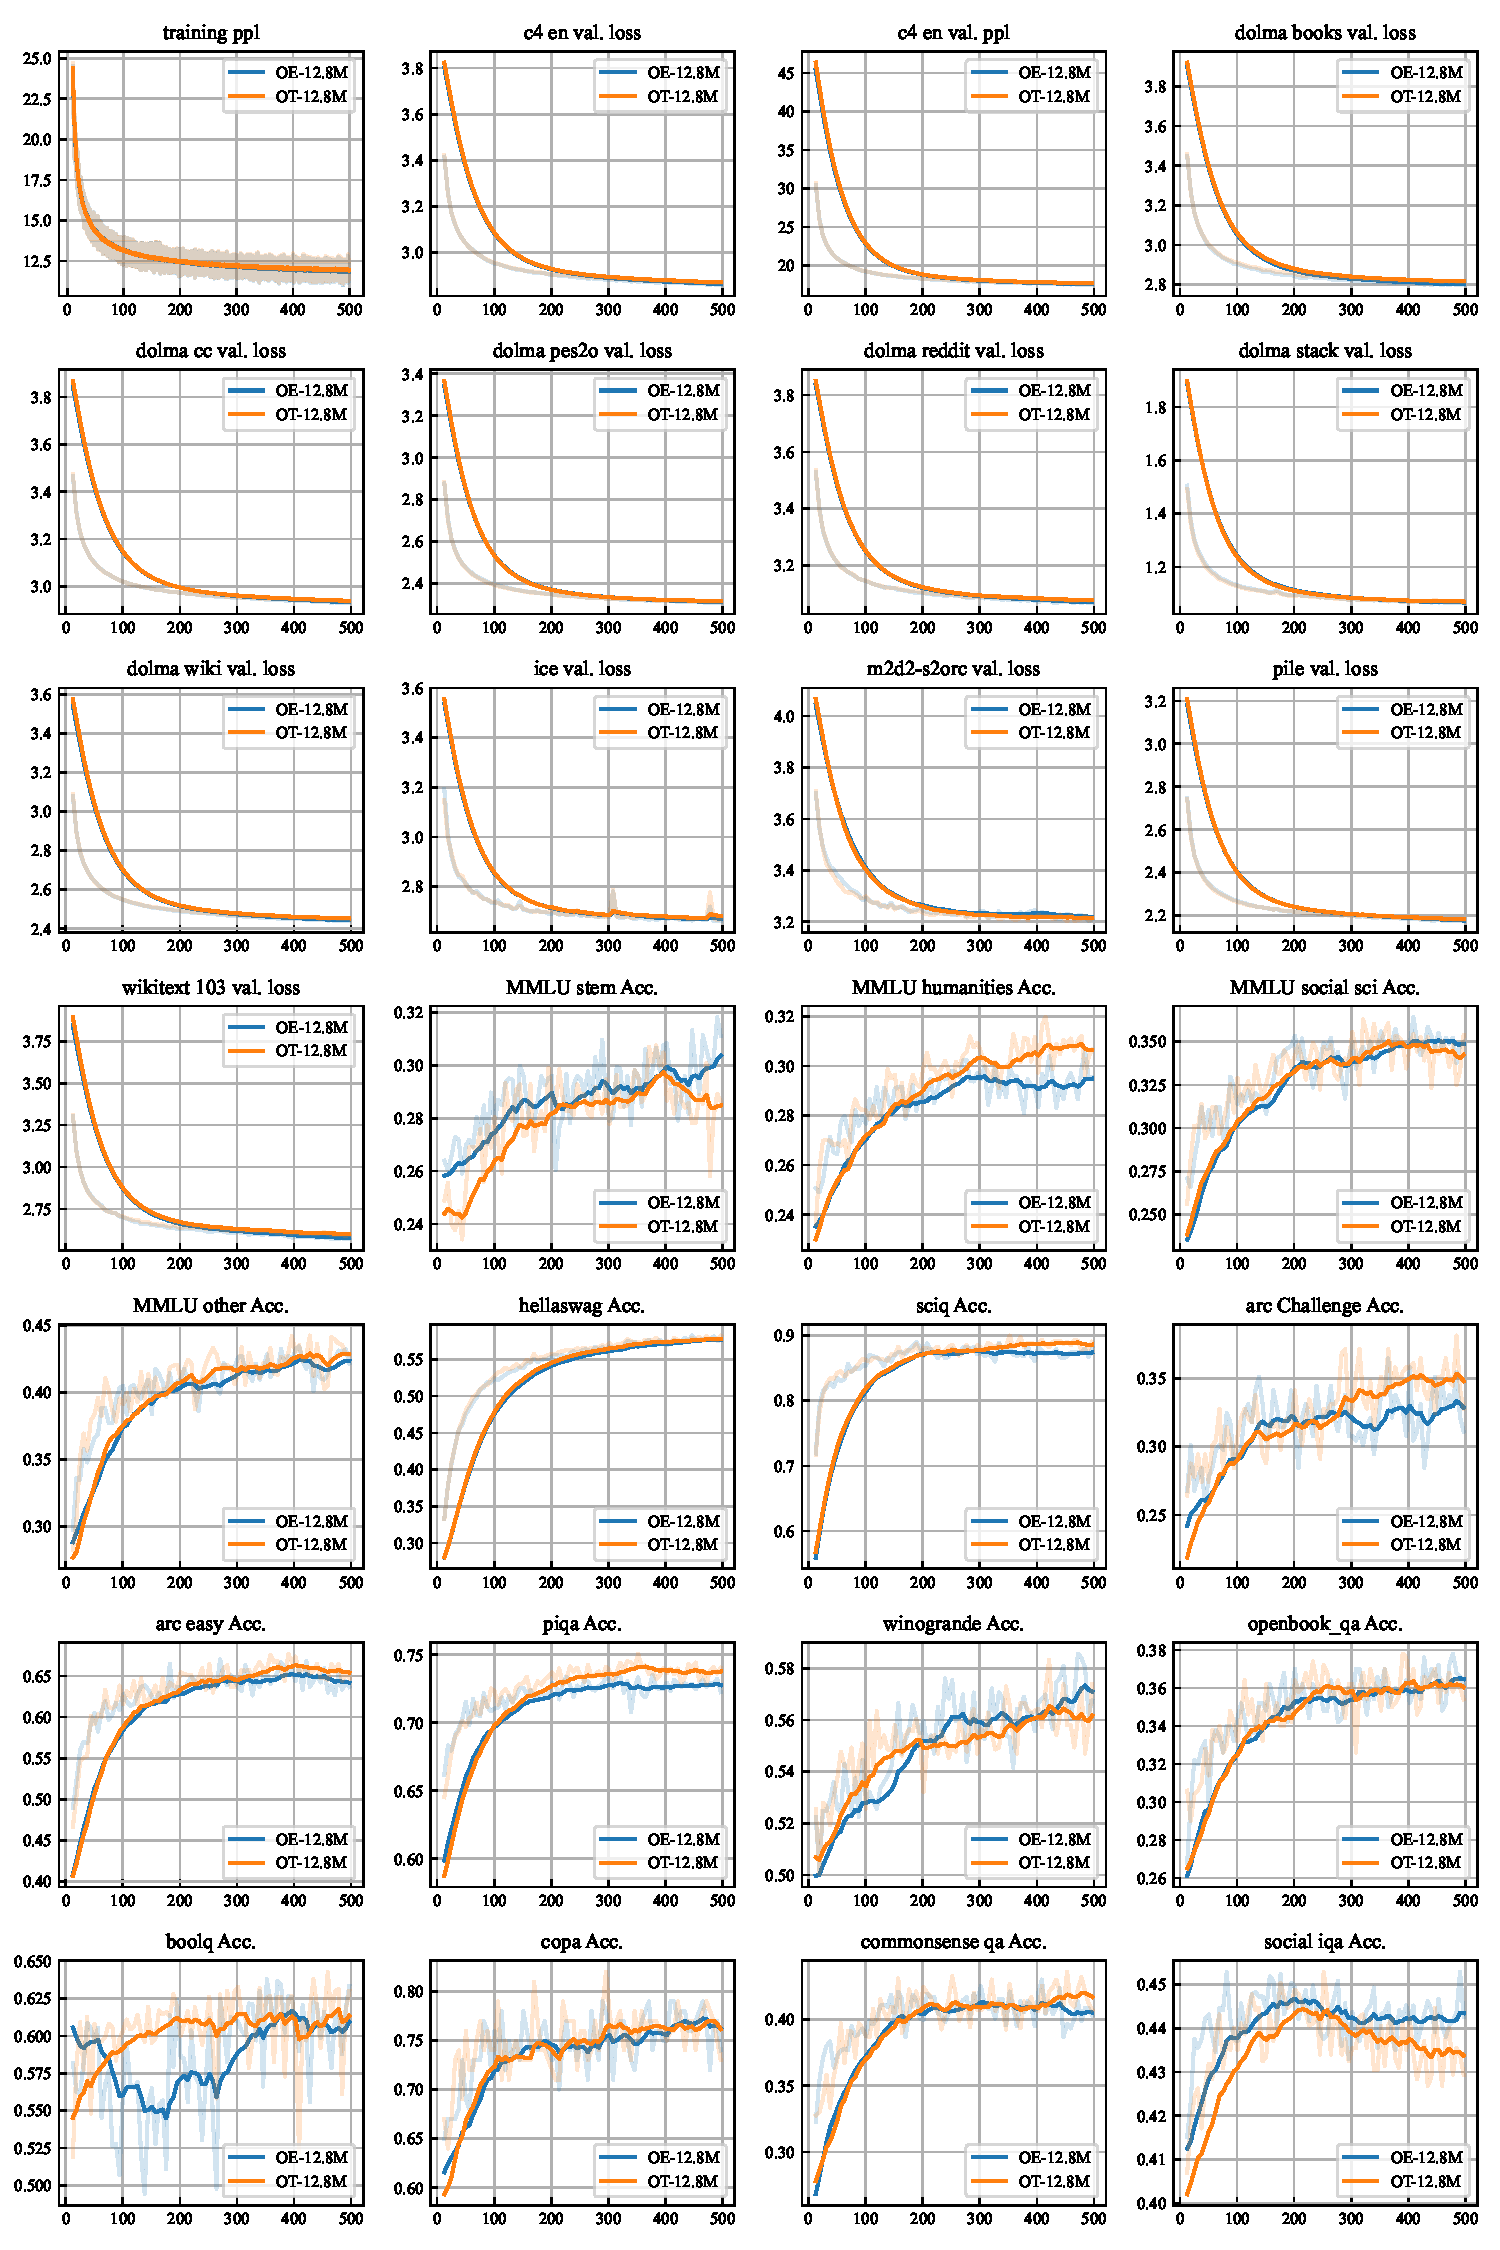
\includegraphics[width=0.85\linewidth]{figures/olmoe_1b3_ot_all_metrics.pdf}
    \caption{All metrics for OLMoE-1.3B, comparing OT-12.8 and OE-12.8M. }
    \label{fig:olmoe_1b3_ot_all_metrics}
\end{figure*}


\paragraph{Loss curves for vocabulary scaling.} We present the loss curves and loss difference curves in \figref{fig:olmoe_scaling_vocab_loss_curves}. The larger input vocabulary requires longer training to obtain all its gains.

\paragraph{Loss curves for OLMoE-7B models.} We present the loss curves for OLMoE-7B in \figref{fig:olmoe_7b_sota_loss_curves}. The gains of OE have not fully converged in 500B tokens' training. Comparing to the experiments on OLMoE-1.3B, it is likely that larger models require more training to fully leverage the power of over-encoding. 

\paragraph{Detailed metrics for OE.} We present a detailed training dynamics comparison for OE-12.8M and baseline model in \figref{fig:olmoe_1b3_oe_all_metrics}(OLMoE-1.3B) and \figref{fig:olmoe_7b_oe_all_metrics}(OLMoE-7B). Our model has significant improvements on most evaluation metrics, and has at least comparable performance for the rest.

\paragraph{Detailed metrics for OT.} We present detailed metrics comparing OT-12.8M and OE-12.8M on OLMoE-1.3B in \figref{fig:olmoe_1b3_ot_all_metrics}. OT is not always better than OE, \eg, Winogrande and Social IQA.


\subsection{In-house Experiments}
We also perform in-house experiments to verify the effectiveness of over-encoding. The in-house baseline adopts MoE architecture, having 400M activated parameters and 4B sparse parameters in total. Then we implement OE, scaling up the vocabulary size to $m=36\mathrm{M}$. We train 600B tokens with in-house pre-training datasets, and evaluate the model through a series of open benchmarks under the few-shot settings. Results are shown in \tabref{tab:in_house_icl_eval}. OE shows significant gains across different domains, including reasoning, knowledge and math ability. Especially, we notice that OE mostly improves knowledge ability. These results demonstrate that OE also improves in-context learning.

\begin{table}[h]
\centering
\caption{Comparison of OE and baseline on in-house models. The models are evaluated on various benchmarks on the few-shot settings. OE improves both reasoning, knowledge and math related benchmarks.}
\label{tab:in_house_icl_eval}

\begin{tabular}{|l|l|l|l|l|l|}
\hline
& \multicolumn{5}{c|}{Reasoning Related Benchmarks} \\ \cline{2-6}
& ARC Challenge & Drop & BBH & WinoGrande & Hellaswag \\ \hline
Baseline & 65.7 & 34.4 & 37.1 & 63.2 & 66.2 \\ \hline
+OE 36M & 67.9 & 36.3 & 39.5 & 65.5 & 67.2 \\ \hline
\end{tabular}

\vspace{10pt}

\begin{tabular}{|l|l|l|l|l|l|}
\hline
& \multicolumn{5}{c|}{Knowledge Related Benchmarks} \\ \cline{2-6}
& MMLU & C-Eval & TriviaQA & MMLU-Pro & AGIEval \\ \hline
Baseline & 54.8 & 61.3 & 39.7 & 21.1 & 39.1 \\ \hline
+OE 36M & 57.9 & 68.3 & 49.0 & 24.1 & 43.2 \\ \hline
\end{tabular}

\vspace{10pt}

\begin{tabular}{|l|l|l|l|}
\hline
& \multicolumn{3}{c|}{Math Related Benchmarks} \\ \cline{2-4}
& Ape210K & GSM8K & MATH \\ \hline
Baseline & 63.7 & 40.6 & 22.7 \\ \hline
+OE 36M & 63.8 & 46.2 & 25.3 \\ \hline
\end{tabular}
\end{table}


\section{Over-Decoding}
\label{appendix:od}

\paragraph{Method.} From previous experiments on synthetic data, we know that an excessively large output vocabulary is detrimental to small models. Therefore, when designing an over-decoding method based on natural language, we aim to leverage the advantages of $n$-gram prediction while keeping the decoding vocabulary size as small as possible. We found that product decomposition provides a promising solution to this problem. 

For the $n$-gram decoding vocabulary, the product embedding decomposition parameterizes a $V^n$-sized embedding table using $n$ separate $V$-sized embedding tables, formulated as:
\begin{equation}
    \tilde{\mathbf{e}}_{x}=\sum_{j=1}^n\mathbb{E}^{V\times d}_j(x/V^{j-1})=\sum_{j=1}^n\mathbf{E}_j(z_{j}),
\end{equation}
where $\tilde{\mathbf{e}}_{x}$ is the reparameterized 2-gram embedding, and $z_1, \dots, z_n$ correspond to the reverse mapping of the function $f$ given $x$, as described in~\refeq{eq:index_mapping_func}. Then, during training,  we compute the next $n$-gram token prediction loss on the reparameterized embeddings $\{\tilde{\mathbf{e}}_i\}$:
\begin{equation}
    \mathcal{L}=\texttt{CE}(\mathbf{\hat{h}}\tilde{\mathbf{E}}^\top, x^{(+n)})=\sum_{j=1}^n\texttt{CE}(\mathbf{\hat{h}}\mathbf{E}_j^\top, z_j), \label{eq:od_loss_decomposition}
\end{equation}
where $\hat{h}$ represents the output hidden state, $\texttt{CE}(\cdot, \cdot)$ denotes the cross-entropy loss, and the loss decomposition is detailed later. 

A notable challenge is that the decoding embedding is densely activated, making the unembedding layer computationally expensive, particularly for smaller models. To address this, we optionally apply a low-rank decomposition by projecting the last hidden state to a smaller dimension. Additionally, we reweigh these losses using a set of hyperparameters $\lambda_1, \dots, \lambda_n$, resulting in the final training loss:
\begin{equation}
    \mathcal{L}=\sum_{j=1}^n\lambda_j\texttt{CE}(\mathbf{\hat{h}}\mathbf{W}_j\mathbf{E}_j^\top, z_j),
\end{equation}
where $\mathbf{W}_j$ is the optional projection matrix corresponding to the $j$-th embedding table. We typically set $\lambda_1=1$ and $\forall i>1, \lambda_i\leq 1$. A pytorch-like implementation is provided in Algorithm~\ref{alg:torch_od_impl}.

\paragraph{Derivation of Loss Decomposition}
We provide a detailed derivation of the loss decomposition in \eqref{eq:od_loss_decomposition}. Recall that $\{\tilde{\mathbf{e}}_i\}$ are the $n$-gram token embedding table. Each of them is reparameterized by $\tilde{\mathbf{e}}_i=\sum_{j=1}^n\mathbf{E}_j(z_{j})$ with $i=\sum_jz_jV^j$. We denote $\mathbf{e}_{z_j}^{(j)}=\mathbf{E}_j(z_{j})$, then $\tilde{\mathbf{e}}_i=\sum_{j=1}^n\mathbf{e}_{z_j}^{(j)}$. Cross-entropy loss using $n$-gram token prediction task on $\{\tilde{\mathbf{e}}_i\}$ can be written as:
\begin{align}
    \mathcal{L}(\hat{\mathbf{h}},x^{(+n)};\tilde{\mathbf{E}}) &=-\log{ 
        \frac{\texttt{exp}(\hat{\mathbf{h}}\tilde{\mathbf{e}}_{x^{(+n)}})}
            {\sum_i\texttt{exp}(\hat{\mathbf{h}}\tilde{\mathbf{e}}_{i})}
        }
        = -\log{ 
        \frac{\texttt{exp}(\hat{\mathbf{h}}(\sum_j\mathbf{e}_{x_j}^{(j)}))}
            {\sum_{z_1,\dots,z_n}\texttt{exp}(\hat{\mathbf{h}}(\sum_j\mathbf{e}_{z_{j}}^{(j)}))}
        } \notag \\
        &= -\log{ 
        \frac{\prod_j \texttt{exp}(\hat{\mathbf{h}}\mathbf{e}_{x_j}^{(j)})}
            {\sum_{z_1,\dots,z_n}\prod_j\texttt{exp}(\hat{\mathbf{h}}\mathbf{e}_{z_{j}}^{(j)})}
        } = -\log{ 
        \frac{\prod_j \texttt{exp}(\hat{\mathbf{h}}\mathbf{e}_{x_j}^{(j)})}
            {\prod_j\left(\sum_{z_j}\texttt{exp}(\hat{\mathbf{h}}\mathbf{e}_{z_{j}}^{(j)})\right)}
        } \notag \\
        &= -\log{ 
            \prod_j\frac{ \texttt{exp}(\hat{\mathbf{h}}\mathbf{e}_{x_j}^{(j)})}
            {\sum_{z_j}\texttt{exp}(\hat{\mathbf{h}}\mathbf{e}_{z_{j}}^{(j)})}
        }= \sum_j-\log{ 
            \frac{ \texttt{exp}(\hat{\mathbf{h}}\mathbf{e}_{x_j}^{(j)})}
            {\sum_{z_j}\texttt{exp}(\hat{\mathbf{h}}\mathbf{e}_{z_{j}}^{(j)})}
        } =\sum_j\mathcal{L}(\hat{\mathbf{h}},x_j; \mathbf{E}_j),
\end{align}
where $x_j$ is the next-$j$ token, and $x^{(+n)}=\sum_jx_jV^{j-1}$. Hence, with product embedding decomposition, the $n$-gram token prediction can be decomposed to multiple next-$j$ token prediction loss, which can be calculated efficiently.


\paragraph{Discussion.} Based on product embedding decomposition, we propose a training objective similar to MTP~\cite{gloeckle2024better}. Formally, we remove the additional transformer layer introduced by the multiple prediction heads in MTP. Instead, we directly decode the next 1 to $n$ tokens from the last hidden state using $n$ different vocabularies. 

From the perspective of MTP, the nonlinear transformation introduced by directly using new vocabularies in the prediction heads is not weaker than adding a transformer layer. Moreover, since the unembedding process is a computational bottleneck, using a new set of parameters does not reduce training throughput compared to MTP.

From the perspective of Over-decoding, we retain the potential to scale up the output vocabularies. This means that the training process provides finer-grained supervision signals, which may enable the model to learn better representations. However, this approach is likely only practical for sufficiently large models. On one hand, larger models have a smaller proportion of computation spent on unembedding. On the other hand, larger models offer greater capacity to take advantage of this setup.


\begin{algorithm}[h]
\caption{Over-Decoding in a PyTorch-like style.}
\label{alg:torch_od_impl}

\definecolor{codeblue}{rgb}{0.25,0.5,0.5}
\definecolor{codekeywd}{rgb}{0,0,1}
\lstset{
  backgroundcolor=\color{white},
  basicstyle=\fontsize{7.2pt}{7.2pt}\ttfamily\selectfont,
  columns=fullflexible,
  breaklines=true,
  captionpos=b,
  commentstyle=\fontsize{7.2pt}{7.2pt}\color{codeblue},
  keywordstyle=\fontsize{7.2pt}{7.2pt}\color{codekeywd},
%  frame=tb,
}
\begin{lstlisting}[language=python]
#OD parameters:
#  n: the number of next tokens involved
#  lambdas: list of n-1 elements, indicating loss weights for next i+1 token pred
#  d: dimension for low-rank decomposition
#Model parameters:
#  V: base vocabulary size
#  D: model dimension

#Torch Modules
wte = nn.Embedding(V, d) # default next 1 token embedding table
od_embs = nn.ModuleList([
    nn.Sequential(
        nn.Linear(D, d) if D != d else nn.Identity(),
        nn.Linear(d, V)
    ) 
    for i in range(n-1)])
ce_loss = nn.CrossEntropyLoss()

def forward(self, input_ids, hidden_states):
    # input_ids: [bs, seqlens]
    # hidden_states: [bs, seqlens, D]
    loss = ce_loss(F.linear(hidden_states[:,:-1], wte.weight.T), input_ids[:,1:])
    for i in range(2, n+1):
        loss += lambdas[i-2] * ce_loss(od_embs[i-2](hidden_states[:-i]), input_ids[:,i:])
    return loss

\end{lstlisting}
\end{algorithm}



\subsection{Experiments}


\begin{figure*}
    \centering
    \subfigure[OLMoE-1.3B]{
        \label{fig:}
	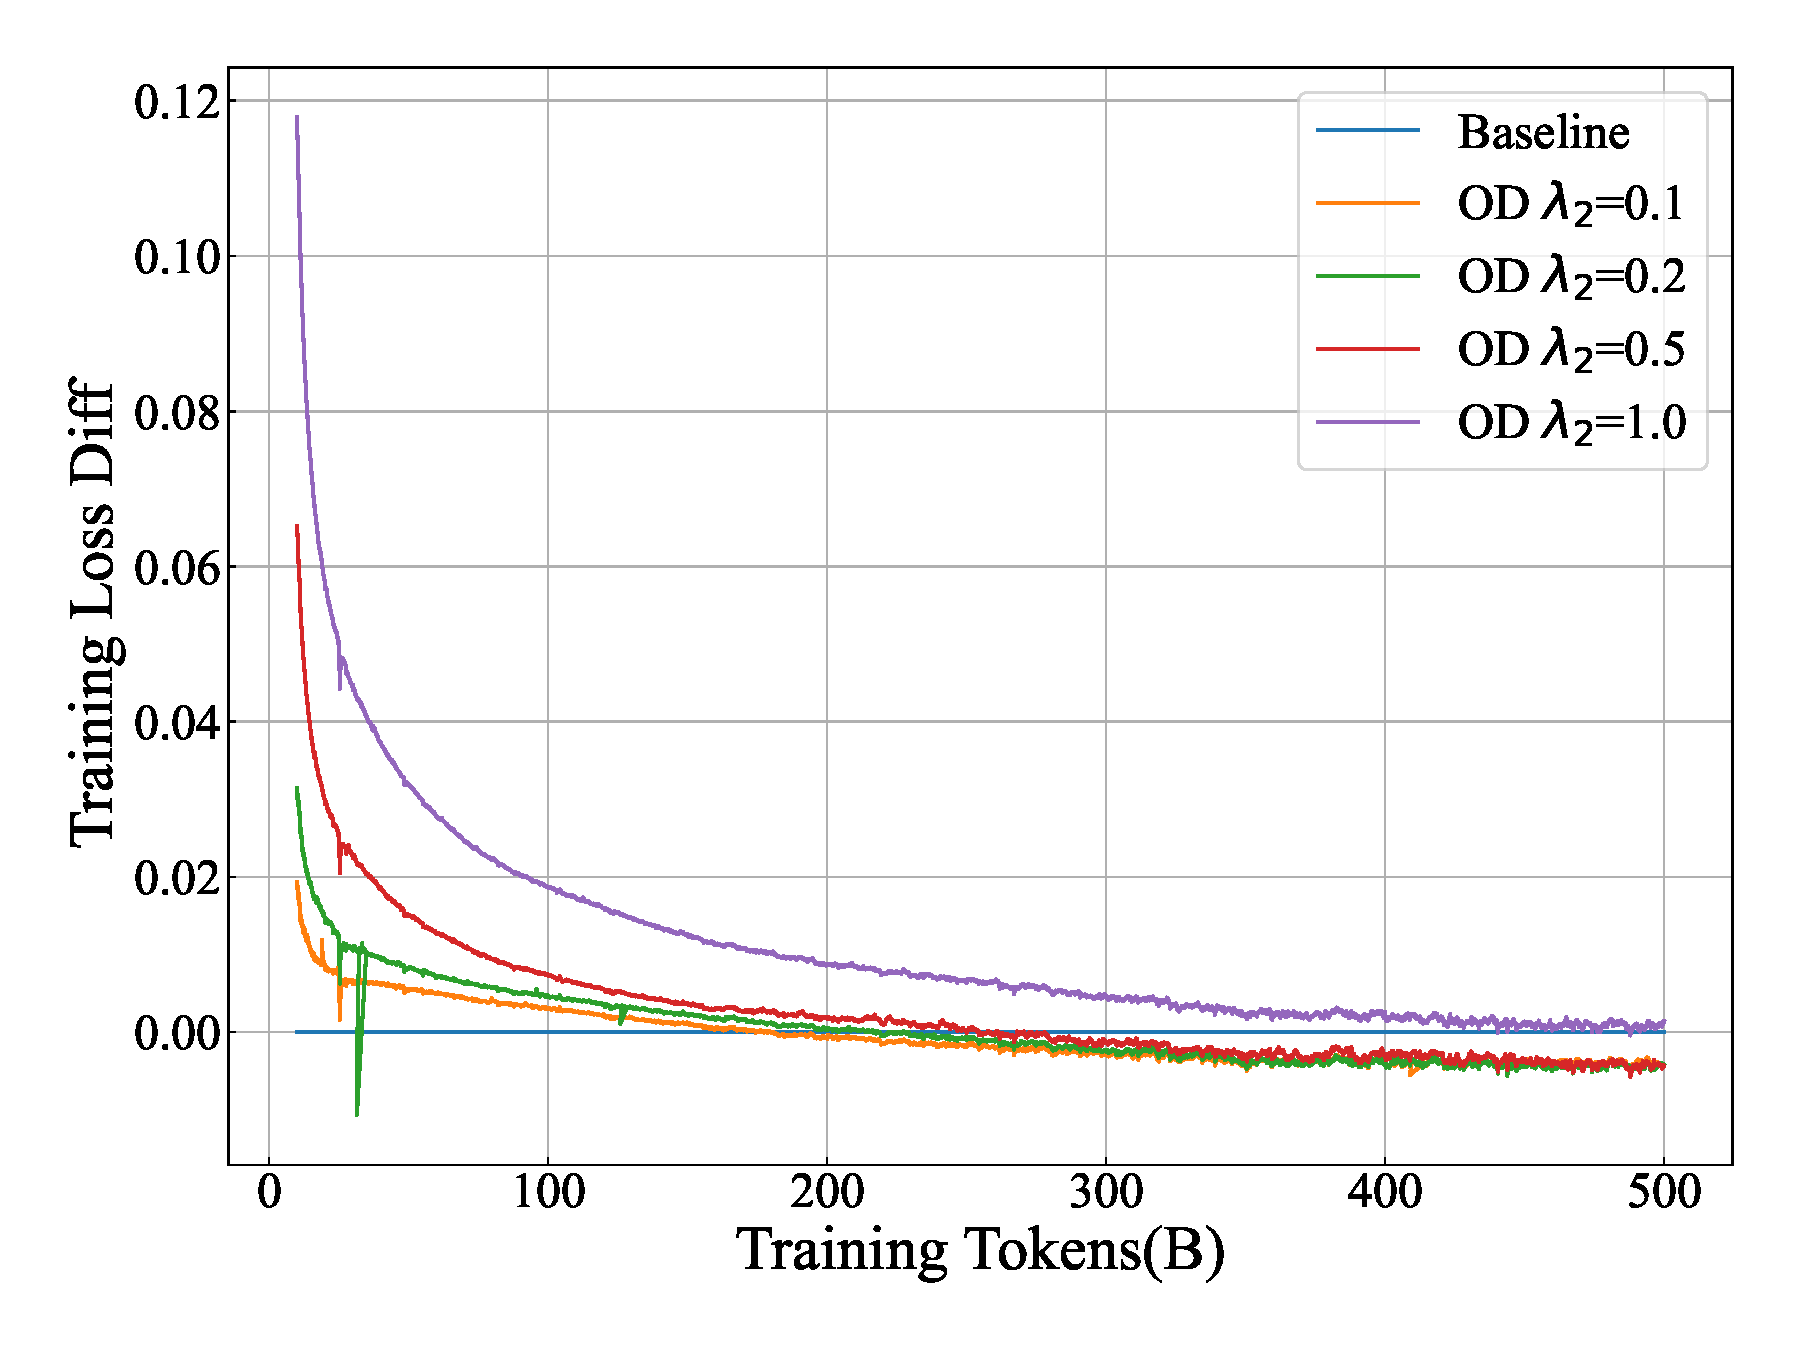
\includegraphics[width=0.45\linewidth]{figures/olmoe_1b3_od_loss_diff.pdf}
	}
    \subfigure[OLMoE-7B]{
        \label{fig:}
	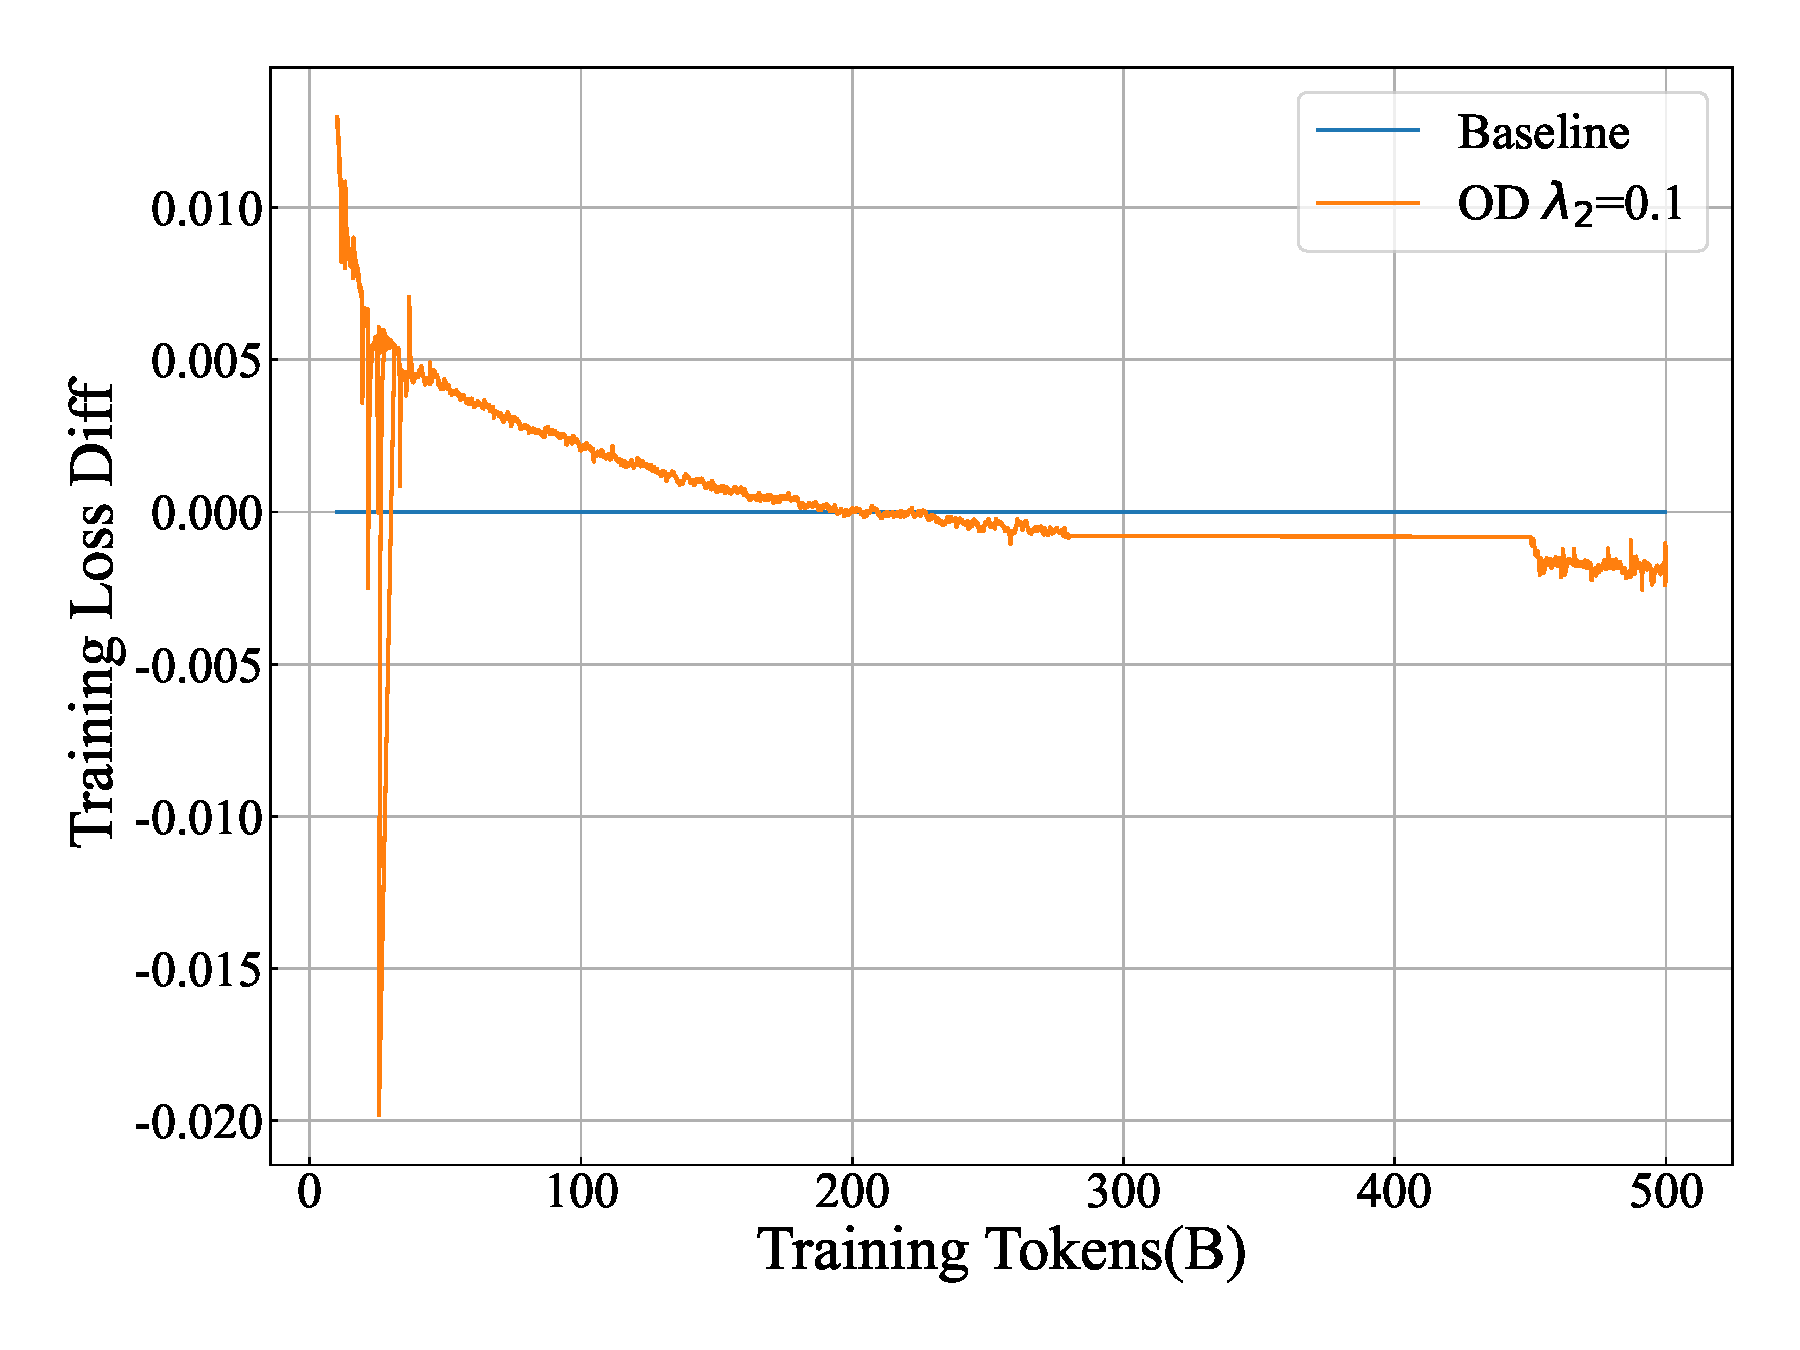
\includegraphics[width=0.45\linewidth]{figures/olmoe_7b_od_loss_diff.pdf}
	}
    \caption{Loss diff curves comparing over-decoded models and baselines. OD models use the setting of $n=2$ and $\lambda_2\in[0.1,0.2,0.5,1.0]$. The curves are smoothed with exponential moving average of weight $0.99$. }
    \label{fig:olmoe_od_loss_diff_curves}
\end{figure*}

We conduct experiments for Over-Decoding under OLMoE settings, where both OLMoE-1.3B and OLMoE-7B are considered. We train 500B tokens for all the experiments.

\paragraph{OD improves baseline with sufficient training.}
We first observed that over-decoding significantly lags behind the baseline in the early stages of training. However, after training on more than 200B tokens, over-decoding begins to outperform the baseline. This experiment is conducted on both 1.3B and 7B OLMoE models, where we set $n=2$. As shown in \figref{fig:olmoe_od_loss_diff_curves}, the next-one-token loss for over-decoding surpasses the baseline with a steeper slope. Downstream metrics, as illustrated in \tabref{tab:ablation_od_weights}, also show slight improvements with proper loss weight choosen. Typically, we find training loss converges to similar values regardless of loss weights. But from the downstream tasks, a smaller weight leads to better overall performance. 


\begin{table}
\centering
\caption{Ablation study on loss weights for OD. The column downstream represents the average score of MMLU-Var, Hellaswag, ARC-Challenge, ARC-Easy and PIQA. }
\begin{tabular}{c|ccccccc}
\toprule
Model & Loss$\downarrow$ & Eval Loss$\downarrow$ & MMLU-Var$\uparrow$ & Hellaswag$\uparrow$ & Arc-Challenge$\uparrow$ & Arc-Easy$\uparrow$ & PIQA$\uparrow$ \\ \midrule
OLMoE-1.3B          & 2.554 & 2.924 & 0.327 & \textbf{0.553} & 0.325 & 0.622 & 0.727 \\
+OD $\lambda_2=0.1$ & 2.549 & 2.920 & 0.325 & \textbf{0.553} & \textbf{0.331} & 0.610 & 0.721 \\
+OD $\lambda_2=0.2$ & 2.549 & \textbf{2.918} & 0.327 & 0.551 & 0.323 & \textbf{0.633} & \textbf{0.728} \\
+OD $\lambda_2=0.5$ & 2.549 & \textbf{2.918} & 0.325 & \textbf{0.553} & 0.308 & 0.619 & 0.727 \\
+OD $\lambda_2=1.0$ & 2.555 & 2.923 & \textbf{0.328} & 0.550 & 0.320 & 0.629 & 0.722 \\
\midrule
OLMoE-7B            & 2.306 & \textbf{2.670} & 0.385 & \textbf{0.695} & \textbf{0.414} & \textbf{0.740} & 0.775  \\
+OD $\lambda_2=0.1$ & \textbf{2.304} & 2.672 & \textbf{0.387} & 0.691 & 0.409 & 0.724 & \textbf{0.776} \\
\bottomrule
\end{tabular}
\label{tab:ablation_od_weights}
\end{table}
